% !BIB TS-program = biber

\RequirePackage[l2tabu,orthodox]{nag}

\documentclass[headsepline,footsepline,footinclude=false,fontsize=11pt,paper=a4,listof=totoc,bibliography=totoc,BCOR=12mm,DIV=12]{scrbook} % two-sided
% \documentclass[headsepline,footsepline,footinclude=false,oneside,fontsize=11pt,paper=a4,listof=totoc,bibliography=totoc]{scrbook} % one-sided

\PassOptionsToPackage{table,svgnames,dvipsnames}{xcolor}

\usepackage[utf8]{inputenc}
\usepackage[T1]{fontenc}
\usepackage[sc]{mathpazo}
\usepackage[american]{babel}
\usepackage[autostyle]{csquotes}
\usepackage[%
  backend=biber,
  url=true,
  sorting=none,
  style=numeric-comp,
  maxnames=4,
  minnames=3,
  maxbibnames=99,
  giveninits,
  uniquename=init]{biblatex}
\usepackage{graphicx}
\usepackage{subcaption}
\usepackage{tabularray}
\UseTblrLibrary{booktabs}
\usepackage{mathtools}
\usepackage{scrhack} % necessary for listings package
\usepackage{listings}
\usepackage{lstautogobble}
\usepackage{tikz}
\usepackage{pgfplots}
\usepackage{pgfplotstable}
\usepackage{booktabs}
\usepackage[final]{microtype}
\usepackage{caption}
\usepackage[printonlyused]{acronym}
\usepackage[hidelinks]{hyperref} % hidelinks removes colored boxes around references and links
\AtBeginDocument{%
	\hypersetup{
		pdftitle=\getTitle,
		pdfauthor=\getAuthor,
	}
}
\usepackage{ifthen}

\addto\extrasamerican{
	\def\lstnumberautorefname{Line}
	\def\chapterautorefname{Chapter}
	\def\sectionautorefname{Section}
	\def\subsectionautorefname{Subsection}
	\def\subsubsectionautorefname{Subsubsection}
}

\addto\extrasngerman{
	\def\lstnumberautorefname{Zeile}
}

% Themes
\ifthenelse{\equal{\detokenize{dark}}{\jobname}}{%
  % Dark theme
  \newcommand{\bg}{black} % background
  \newcommand{\fg}{white} % foreground
  \usepackage[pagecolor=\bg]{pagecolor}
  \color{\fg}
}{%
  % Light theme
  \newcommand{\bg}{white} % background
  \newcommand{\fg}{black} % foreground
}

\bibliography{bibliography}

\setkomafont{disposition}{\normalfont\bfseries} % use serif font for headings
\linespread{1.05} % adjust line spread for mathpazo font

% Add table of contents to PDF bookmarks
\BeforeTOCHead[toc]{{\cleardoublepage\pdfbookmark[0]{\contentsname}{toc}}}

% Define TUM corporate design colors
% Taken from http://portal.mytum.de/corporatedesign/index_print/vorlagen/index_farben
\definecolor{TUMBlue}{HTML}{0065BD}
\definecolor{TUMSecondaryBlue}{HTML}{005293}
\definecolor{TUMSecondaryBlue2}{HTML}{003359}
\definecolor{TUMBlack}{HTML}{000000}
\definecolor{TUMWhite}{HTML}{FFFFFF}
\definecolor{TUMDarkGray}{HTML}{333333}
\definecolor{TUMGray}{HTML}{808080}
\definecolor{TUMLightGray}{HTML}{CCCCC6}
\definecolor{TUMAccentGray}{HTML}{DAD7CB}
\definecolor{TUMAccentOrange}{HTML}{E37222}  % Software
\definecolor{TUMAccentGreen}{HTML}{A2AD00}
\definecolor{TUMAccentLightBlue}{HTML}{98C6EA}
\definecolor{TUMAccentBlue}{HTML}{64A0C8}    % Hardware

% Settings for pgfplots
\pgfplotsset{compat=newest}
\pgfplotsset{
  % For available color names, see http://www.latextemplates.com/svgnames-colors
  cycle list={TUMBlue\\TUMAccentOrange\\TUMAccentGreen\\TUMSecondaryBlue2\\TUMDarkGray\\},
}

% Settings for lstlistings
\lstset{%
  basicstyle=\ttfamily,
  columns=fullflexible,
  autogobble,
  keywordstyle=\bfseries\color{TUMBlue},
  stringstyle=\color{TUMAccentGreen},
  captionpos=b
}


\newcommand*{\getUniversity}{Technische Universität München}
\newcommand*{\getFaculty}{Informatics}
\newcommand*{\getDegree}{Informatics}
\newcommand*{\getSchool}{Computation, Information and Technology}
\newcommand*{\getTitle}{Establishing Trust in an Updatable fTPM Using Remote
Attestation}
\newcommand*{\getTitleGer}{Herstellung von Vertrauen in ein aktualisierbares fTPM durch Remote Attestierung}
\newcommand*{\getAuthor}{Andreas Korb}
\newcommand*{\getDoctype}{Master's Thesis}
\newcommand*{\getSupervisor}{Prof.\ Dr.\ Claudia Eckert}
\newcommand*{\getAdvisor}{Albert Stark, Johannes Wiesböck}
\newcommand*{\getSubmissionDate}{15.01.2024}
\newcommand*{\getSubmissionLocation}{Munich}

\begin{document}

% Set page numbering to avoid "destination with the same identifier has been already used" warning for cover page.
% (see https://en.wikibooks.org/wiki/LaTeX/Hyperlinks#Problems_with_Links_and_Pages).
\pagenumbering{alph}
\input{pages/cover}

\frontmatter{}

\begin{titlepage}
  \centering

  \IfFileExists{logos/tum-\fg.pdf}{%
    \includegraphics[height=20mm]{logos/tum-\fg.pdf}
  }{%
    \vspace*{20mm}
  }

  \vspace{5mm}
  {\huge\MakeUppercase{School of \getSchool{} --- \getFaculty{}} \par}

  \vspace{5mm}
  {\large\MakeUppercase{\getUniversity{}} \par}

  \vspace{20mm}
  {\Large \getDoctype{} in \getDegree{} \par}

  \vspace{15mm}
  {\huge\bfseries \getTitle{} \par}

  \vspace{10mm}
  {\huge\bfseries \foreignlanguage{ngerman}{\getTitleGer{}} \par}

  % TODO Verify whether setting 10mm instead of 15mm here is okay
  \vspace{10mm}
  \begin{tabular}{l l}
    Author:          & \getAuthor{}         \\
    Supervisor:      & \getSupervisor{}     \\
    Advisor:         & \getAdvisor{}        \\
    Submission Date: & \getSubmissionDate{} \\
  \end{tabular}

  \IfFileExists{logos/faculty-\fg.pdf}{%
    \vfill{}
    \includegraphics[height=20mm]{logos/faculty-\fg.pdf}
  }{}
\end{titlepage}

\thispagestyle{empty}
\vspace*{0.8\textheight}
\noindent
I confirm that this \MakeLowercase{\getDoctype{}} is my own work and I have documented all sources and material used.

\vspace{15mm}
\noindent
\getSubmissionLocation{}, \getSubmissionDate{} \hspace{\fill} \getAuthor{}

\cleardoublepage{}

\addcontentsline{toc}{chapter}{Acknowledgments}
\thispagestyle{empty}

\vspace*{20mm}

\begin{center}
    {\usekomafont{sectioning}\usekomafont{section} Acknowledgments}
\end{center}

\vspace{10mm}

I would like to take this opportunity to thank all those who have supported me in the preparation of this thesis.
My thanks go to my supervisor Prof.\ Dr.\ Claudia Eckert, who gave me the opportunity to write this thesis.
I would also like to express my special thanks to my advisors Albert Stark and Johannes Wiesböck, who patiently stood by my side and answered all my questions.
Without their help and support, this thesis would not have been possible, and I am sure they have helped me greatly to start my journey in the field of cyber security.
Last but not least, I would like to thank all my friends who have been patient and understanding during the writing of this thesis and who have sacrificed their time to proofread my work.


\cleardoublepage{}

\chapter{\abstractname}

Zero Trust is a cybersecurity paradigm in which a network, e.g., an enterprise network, is considered compromised.
Therefore, each device of every service request must be verified before the request is served.
This is made possible by remote attestation, which is enabled by TPMs, for example.
For that, they authenticate themselves by propagating their so-called endorsement certificate naming their manufacturer, who guarantees they conform to the TPM specification to ensure their security properties.
While this approach is sufficient for hardware TPMs as they are standalone chips, for firmware TPMs~(fTPM) it is assumed that the manufacturer of the fTPM is the same as that of all firmware components that were booted before the fTPM\@.
This is due to the fact that any previous firmware component can compromise the fTPM during loading.
The verifier in the remote attestation procedure lacks the ability of verifying the entire boot chain up to the fTPM\@.
We propose a remote attestation system that provides the verifier with this possibility.
To compensate for the lack of a hardware root of trust of an fTPM compared to a hardware TPM, we introduce DICE as the hardware root of trust.
The verifier only needs to trust the manufacturer of DICE, while every firmware component beyond is explicitly attested by passing their identities to the verifier.
The three benefits of our solution are that (i) the manufacturer of the fTPM and its preceding firmware components can be independent of each other, (ii) detection of modification of fTPM by remote verifier, and (iii) protection of the fTPM's data-at-rest.
% Explain (ii)
DICE measures the first firmware component, which is then repeated up to the fTPM\@.
These measurements are forwarded to the remote verifier, which can then detect potentially malicious changes to each measured component.
% Explain (iii)
The fTPM's data-at-rest is protected by binding it to the identity of the fTPM\@.
This means that the data of an fTPM is only accessible to the fTPM that created it as long as its identity does not change, which makes downgrade attacks and changes to the fTPM less attractive to attackers.

\microtypesetup{protrusion=false}
\tableofcontents{}
\microtypesetup{protrusion=true}

\mainmatter{}

\acresetall{}

%% !TeX root = ../main.tex
% Add the above to each chapter to make compiling the PDF easier in some editors.

\chapter{Template examples}

\section{Section}
Citation test~\parencite{latex}.

Acronyms must be added in \texttt{main.tex} and are referenced using macros. The first occurrence is automatically replaced with the long version of the acronym, while all subsequent usages use the abbreviation.

E.g. \texttt{\textbackslash ac\{TUM\}, \textbackslash ac\{TUM\}} $\Rightarrow$ \ac{TUM}, \ac{TUM}

For more details, see the documentation of the \texttt{acronym} package\footnote{\url{https://ctan.org/pkg/acronym}}.
\subsection{Subsection}

See~\autoref{tab:sample}, \autoref{fig:sample-drawing}, \autoref{fig:sample-plot}, \autoref{fig:sample-listing}.

\begin{table}[htpb]
  \caption[Example table]{An example for a simple table.}\label{tab:sample}
  \centering
  \begin{tabular}{l l l l}
    \toprule
      A & B & C & D \\
    \midrule
      1 & 2 & 1 & 2 \\
      2 & 3 & 2 & 3 \\
    \bottomrule
  \end{tabular}
\end{table}

\begin{figure}[htpb]
  \centering
  % This should probably go into a file in figures/
  \begin{tikzpicture}[node distance=3cm]
    \node (R0) {$R_1$};
    \node (R1) [right of=R0] {$R_2$};
    \node (R2) [below of=R1] {$R_4$};
    \node (R3) [below of=R0] {$R_3$};
    \node (R4) [right of=R1] {$R_5$};

    \path[every node]
      (R0) edge (R1)
      (R0) edge (R3)
      (R3) edge (R2)
      (R2) edge (R1)
      (R1) edge (R4);
  \end{tikzpicture}
  \caption[Example drawing]{An example for a simple drawing.}\label{fig:sample-drawing}
\end{figure}

\begin{figure}[htpb]
  \centering

  \pgfplotstableset{col sep=&, row sep=\\}
  % This should probably go into a file in data/
  \pgfplotstableread{
    a & b    \\
    1 & 1000 \\
    2 & 1500 \\
    3 & 1600 \\
  }\exampleA
  \pgfplotstableread{
    a & b    \\
    1 & 1200 \\
    2 & 800 \\
    3 & 1400 \\
  }\exampleB
  % This should probably go into a file in figures/
  \begin{tikzpicture}
    \begin{axis}[
        ymin=0,
        legend style={legend pos=south east},
        grid,
        thick,
        ylabel=Y,
        xlabel=X
      ]
      \addplot table[x=a, y=b]{\exampleA};
      \addlegendentry{Example A};
      \addplot table[x=a, y=b]{\exampleB};
      \addlegendentry{Example B};
    \end{axis}
  \end{tikzpicture}
  \caption[Example plot]{An example for a simple plot.}\label{fig:sample-plot}
\end{figure}

\begin{figure}[htpb]
  \centering
  \begin{tabular}{c}
  \begin{lstlisting}[language=SQL]
    SELECT * FROM tbl WHERE tbl.str = "str"
  \end{lstlisting}
  \end{tabular}
  \caption[Example listing]{An example for a source code listing.}\label{fig:sample-listing}
\end{figure}

% !TeX root = ../main.tex
% Add the above to each chapter to make compiling the PDF easier in some editors.

\chapter{Introduction}\label{chapter:introduction}

This chapter explains the problem we are addressing, why, a brief overview of our solution, and the attacks we are trying to fend off.

% nicht wissenschaftliche Teil, zero trust ist jetzt ein Ding, immer mehr embedded ohne TPM (z.B. Gartner Studien)

\section{Motivation}

% Which area this thesis is talking about (Zero Trust)

Modern trust relationships, such as Zero Trust~\cite{isaca2021}, require trustworthy platforms to reliably report their system state.
In such models, trust is no longer implicitly assumed, e.g., by the fact that a device is located within the boundaries of a company.
Instead, each device is considered compromised until proven otherwise on a per-request basis for resources (e.g., printers) and data access~\cite{Rose2020}.

% Primer on remote attestation

This is solved by remote attestation.
In the simplest case, there is a prover and a verifier, as depicted in \autoref{fig:ra_simple}.
The challenge is that the verifier observes nothing but bytes from the prover, and while a benign prover will tell the truth about its state, a compromised prover will lie about its state and claim a trustworthy one.
Therefore, the verifier must establish trust in a helper component on the prover's side.
In a typical setup, this component is immutable without the involvement of its manufacturer, which reveals itself to a verifier by signing and storing a certificate on the helper components supplied by it.
This allows the verifier to establish trust in the helper component by knowing its manufacturer.
Consequently, the component attests to the state of the prover's machine, from which the verifier can deduce whether the prover can be considered trustworthy.

\begin{figure}[htpb]
  \centering
  \includegraphics[width=0.5\linewidth]{figures/remote_attestation_process.pdf}
  \caption{Simplified remote attestation process.}\label{fig:ra_simple}
\end{figure}


% TPMs become more important

For example, this can be done with a \ac{TPM} on the prover's side. They rise in their deployments and importance, e.g., in 2013, the President's Council of Advisors on Science and Technology encouraged the adoption of TPMs~\cite{usa}, and Microsoft publicized that they require a TPM module for Windows~11 in 2021~\cite{win11req}.
They provide remote attestation mechanisms of system states, and their applications are still expanding beyond their traditional use cases. For example, they are used in anti-cheat software for games~\cite{valorant}.

% Short intro on why fTPMs were introduced (for weak devices, exactly our target platform)

A \ac{dTPM} increases cost and hardware complexity---especially for embedded platforms.
\Acp{fTPM} running in a \acp{TEE} can be used to provide similar security guarantees as a \ac{dTPM} chip.

% Why establishing trust in an fTPM is harder than in a dTPM

For a \ac{dTPM}, which consists of an independent hardware unit manufactured by a single manufacturer, it is sufficient to identify its manufacturer and understand their provided guarantees.
In contrast, an \ac{fTPM} runs atop other firmware components and is started later in the boot chain, making its security dependent on the underlying firmware stack.
Consequently, trust in an \ac{fTPM} depends on trusting the entire stack beneath it because its underlying firmware might alter or compromise the \ac{fTPM}.

% What's the difficulty of establishing trust in an fTPM?

However, while a TPM-compliant component provides an infrastructure with which trust in it can be established remotely, i.e., an endorsement (key) certificate~(EKcert), this does not represent the underlying firmware stack.

% How it currently works for fTPMs

Currently, this is solved by the manufacturer providing not only the fTPM, but also the entire underlying firmware stack.
Consequently, by establishing trust in the manufacturer of the fTPM, one can implicitly trust the underlying firmware by assuming they also originate from this manufacturer.
This is possible since, in the most general sense, one can derive from an endorsement certificate the endorser, i.e., manufacturer.
If the attester trusts the manufacturer and its provided guarantees, trust is established in its provided components.

\begin{figure}[htpb]
  \centering
  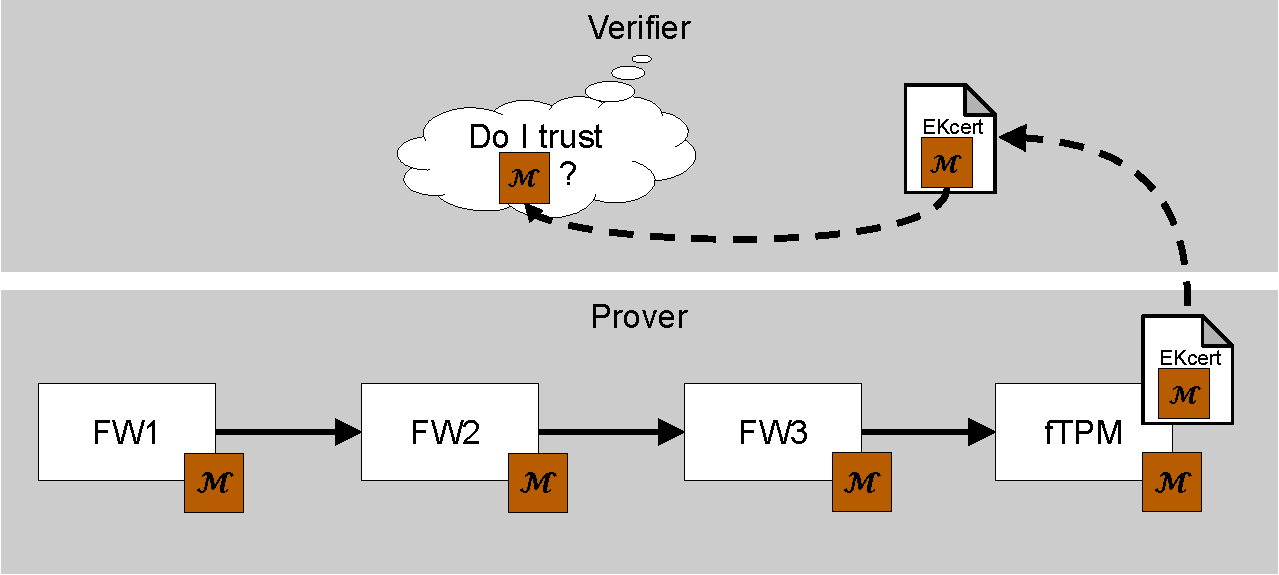
\includegraphics[width=1\linewidth]{figures/current_state.pdf}
  \caption{The naive process how a verifier establishes trust to an \ac{fTPM}, which is in fact done by trusting its manufacturer. The brown markers indicate a manufacturer. The firmware~(FW) and the fTPM were built by manufacturer \(\mathcal{M}\), and the EK certificate indicates this manufacturer.}\label{fig:current_state}
\end{figure}


This process is illustrated in figure \autoref{fig:current_state}.
The prover's box shows its boot chain, and the verifier's box shows how it evaluates the trustworthiness against the prover's boot chain.
The verifier trusts the entire firmware chain if it trusts the manufacturer of each component.
Note how the verifier must assume that the manufacturer of the firmware components is the same as that of the fTPM\@.
To the best of our knowledge, this is what manufacturers like Intel and AMD implement for their \acp{fTPM}, as confidence in their \acp{fTPM} is also only established through an EKcert~\cite{Ruan2014}.

% Summary with limitations

In summary, with the current approach, the endorser, usually a CPU manufacturer, provides the firmware up to the fTPM and guarantees the firmware is not modifiable by untrusted parties.
This enables trust in the other firmware components this manufacturer provided without knowing the firmware.
This approach is limited, as with this mechanism, independent verifiers have to unquestioningly trust the firmware manufacturer, drastically limiting trust relationships.

\section{Goal}

We establish an independently verifiable fTPM stack, rooted in a hardware root of trust, that can be leveraged in a Zero Trust environment with few hardware requirements and without compromising security.
This approach aims to break the requirement of the underlying firmware and the fTPM to originate from the same manufacturer by providing the exact firmware component identities to the verifier, such that it can decide whether they are trustworthy without relying on its manufacturer.
Instead, it is sufficient to trust the independent manufacturer of the hardware root of trust, which requires minimal assumptions, such as the absence of side-channel vulnerabilities.

% Short introduction to DICE

One mechanism enabling firmware attestation is the \ac{DICE}, focusing on resource-constrained devices.
Although this mechanism shifts trust from the firmware provider to the hardware provider by allowing firmware attestation through a hardware root of trust, the exclusive use of this integrated solution is unsuitable for large dynamic systems, such as Linux-based devices.
Nevertheless, the advantage is that the identity of each component of the firmware boot chain is represented.

% How we try to overcome these limitations

We propose a hybrid solution, combining the advantages of \ac{DICE} and \acp{fTPM}, yielding an independently verifiable certificate chain representing the boot chain up to and including the \ac{fTPM}.
This enables a verifier to establish trust in an \ac{fTPM} if the underlying firmware is also benign, thus providing a way to independently assess the properties of the \ac{fTPM}.
% The conceptual basis for this is to attest to the software stack of the TPM itself, thus providing a way to assess the properties of the fTPM independently.

%Current \ac{fTPM} implementations require additional security measures to not leak state between reboots and different software versions.
%The final concept should provide comprehensive guidelines for implementing an fTPM, which accounts for such an environment and reflects any relevant information through remote attestation.

The research questions we aim to answer are listed below.
\begin{enumerate}[label=\textbf{RQ-\arabic*}]
  \item What constitutes the identity of an fTPM\@?\label{rq:1-tpm-identity} %(e.g., hash, configuration, boot chain)
  \item How to combine the DICE and TPM infrastructure?\label{rq:2-combine-infrastructure} %(e.g., AliasCert $\cup$ EKcert)
  \item How to manage an fTPM's persistent data securely?\label{rq:3-secure-data} %(e.g., flush data on update)
  \item How to enable privacy in this attestation mechanism for the prover?\label{rq:4-privacy}
\end{enumerate}

% Prover and verifier can take both roles for mutual attestation

% Chaining the underlying firmware identities with the endorsement identity

\section{Threat Model}

% https://trustedfirmware-a.readthedocs.io/en/latest/threat_model/threat_model.html

% Attacker model: What an attacker can do (abilities) and cannot do (limits)

The attacker we are interested in can replace the fTPM or one of its predecessor components.
Therefore, there is a risk that a remote party trusts a firmware TPM that is not trustworthy.
For example, an attacker could install a malicious update of a relevant firmware component on the target device.
However, we assume the attacker can only do this before or during the device's boot process but not afterward.
Hardware, side-channel, control-flow, and denial-of-service attacks are out-of-scope.

For the network, we assume the Dolev-Yao attacker model~\cite{Dolev1983}, wherein an attacker can perform any active or passive attack on the network.
The attacker may also control parts or the entire network, e.g., all routers, switches, and connections.
Last, they cannot break cryptographic primitives, e.g., encryption, signing, and hashing.

\section{Security goals}

In this section, we want to formally describe the security goals of our solution so that we can later briefly discuss whether and how we achieve the corresponding objectives.

\begin{enumerate}[label=\textbf{SG-\arabic*}]
  \item{\textbf{Compromised fTPM cannot fake its identity}\\
  It is sufficient for a fake identity to be recognized by the verifier, who can consequently classify the prover's fTPM as untrustworthy.}\label{sg:1}
  % Does not have access to OP-TEE's private key; code in user mode does not have access to data in kernel mode

  \item{\textbf{Small root of trust}\\
  A small root of trust, e.g., in code size, hardware size, and complexity, bears less risk in implementation errors, directly affecting security~\cite{Singaravelu2006}.
  % and complexity, and its approaches to guarantee specific security properties are more manageable.
  }\label{sg:2}
  % DICE, its design, not concrete HW, its protection of the \ac{UDS}
  
  \item{\textbf{Isolation of fTPM storage}\\
  Data must only be accessible or modifiable within the boundaries of the fTPM's access controls, i.e., the TPM commands defined by its specification~\cite{tpm20}.
  This includes protecting against other trusted applications running in the same \ac{TEE}\@.}\label{sg:3}
  
  \item{\textbf{Protect fTPM data against downgrade attacks on the fTPM}\\
  Data of the fTPM should be sealed to its identity, such that when the fTPM is modified, e.g., by a downgrade attack, even the fTPM cannot access its old data anymore.}\label{sg:4}

  % \item{\textbf{Privacy of remote attestation process}\\
  % The verifier should be able to establish trust in an fTPM without having to know the identity of the fTPM, i.e., its EK\@.}\label{sg:5}
\end{enumerate}

\section{Outline}

In the \nameref{chapter:background}, we provide the knowledge necessary for a better understanding of the subsequent parts of this thesis.
Afterward, we discuss \nameref{chapter:related_work}, i.e., attacks on TPMs to further motivate this work, approaches to hardening TPMs, and work that enables remote attestation similar to ours.
Under \nameref{chapter:methodology}, we explain the concept of our solution and subsequently present our proof-of-concept \nameref{chapter:implementation}.
Finally, we \hyperref[chapter:discussion]{discuss} our design and implementation, rounded off by the \nameref{chapter:future_work_and_conclusion}.

% !TeX root = ../main.tex
% Add the above to each chapter to make compiling the PDF easier in some editors.

\chapter{Background}\label{chapter:background}

This chapter discusses the relevant background knowledge required to understand the remainder of this work.

\section{Trusted execution environment}

One of the core security concepts of operating systems are the privilege levels of processes. Thereby, processes are protected against other processes with the same or lower privilege level. However, they are not protected against more privileged processes. This bears problems for example for cloud computing and edge computing. In cloud computing, other services, the hypervisor, or the cloud provider in general could potentially access sensitive data of the cloud tenant. In edge computing, the edge applications deal with plain text data, while they are potentially running on insecure edge devices. Hence, protection against more privileged processes is desired.

% Global Platform = industry standard

A \ac{TEE} is an integrated hardware extension to processors. Effectively, the execution environment is separated into the \ac{REE} and the \ac{TEE} by hardware. The \ac{REE} runs the common software, e.g., a Linux-based operating system and the applications. The TEE allows code to be executed and memory separately to be used on a device in a hardware-protected manner that ensures a high level of confidentiality and integrity.
% TODO: Which previous technologies?
Previous technologies ensure protection of data-in-transit, and data-at-rest, while \ac{TEE} additionally protects data-in-use.
Since it is integrated into the processor, there is no separate chip required. However, it is common to give the \ac{TEE} a dedicated volatile memory chip, namely the secure RAM~(sRAM), which is ensured to be exclusively accessible to the \ac{TEE} by hardware.

Moreover, the \ac{TEE} commonly follows the same user and kernel space separation as \ac{REE} operating systems. The kernel space is running a trusted OS kernel, and the user space is running the trusted applications.

One such \ac{TEE} is ARM's TrustZone~\cite{ARM09}. It partitions all software and hardware resources of the containing system into the Normal world~(NW) and the Secure world~(SW).
While the SW can access the resources of the SW and the NW, the NW is restricted to its own resources.
Since ARM is the dominant processor architectures for IoT devices with a market share of 86\,\% \cite{eclipse}, many of the approaches in this field of research rely on ARM technology such as TrustZone.
Our approach also leverages TrustZone to enable the execution and the remote attestation of an fTPM.

Other \ac{TEE} technologies are Intel Software Guard Extensions~(SGX), and AMD Secure Encrypted Virtualization~(SEV), in the future also Intel Trusted Domain Extensions~(TDX), and ARM Confidential Computing Architecture~(CCA). Since we focus on the implementation of our concept with ARM TrustZone, we do not go into detail about these other technologies here. However, since our concept is not tied to ARM processors and can also be applied to others, they are mentioned for the sake of completeness.

% TrustZone, Trusted applications are not isolated -> they need to trust each other

% static: ARM TZ
% dynamic: Intel SGX, TDX, AMD SEV


\section{Attestation}
\subsection{Local attestation}
\subsection{Remote attestation}

Remote attestation is a challenge-response protocol initiated by a remote attestor.
The challenge contains a nonce, enforcing a fresh response.
The response must be a proof of the challenged system that it is trustworthy.

TPMs send \ac{PCR} values in the form of a digitally signed quote to a remote attestor.

Remote attestation is the process initiated by a remote trusted party (called ``verifier'') to verify that an end-device (called ``prover'') has not been tampered with. For detecting that, remote attestation generally inspects the following properties of a program: (i) its code and data has been correctly loaded into memory for execution, (ii) its execution has not been redirected in unintended ways at runtime, and (iii) its data has not been maliciously modified at runtime.

A trusted anchor is required on the device to be attested because at least one trusted component is necessary to extract the data from the remote device to be verified. In many cases, TEE's act as a trust anchor because they are hardware-protected, making it an excellent candidate for a trust anchor.

\section{Trusted Platform Module}

A TPM is a specific \ac{HSM} that increases trust in the underlying platform.
They support three main use-cases: secure key generation, remote system attestation, and secure storage. 
% From https://www.usenix.org/system/files/conference/usenixsecurity18/sec18-han.pdf
% Rephrase
Allows remote attestation with \ac{PCR} values in the form of a digitally signed quote to a remote attestor.

% Explain these, and name use-cases (maybe from book)
% secure key generation
% remote system attestation
% secure storage


% Sealing (local attestation)
% EKCert, EK = Unique ID, key in TPM, used for validation
% Binding to TPM (EK)
% Core Root of Trust of Measurement: BIOS extension, trusted hashing
% PCRs
% Attestation: TPM confirms measured state
While TPM~1.2 is limited to SHA-1 hashes which are considered broken \cite{Stevens2017}, TPM~2.0 offers crypto agility and therefore, also allows newer algorithms such as SHA-256. In general, TPM~2.0 is more flexible, and is always turned on, while TPM~1.2 components needed to be turned on manually.

$PCR(i)_{t+1} \coloneqq hash(PCR(i)_t\ \Vert\ new\ measurement),\ PCR(i)_0 \coloneqq 0$

\begin{table}[htpb]
    \caption[PCR table]{The PCR register usages as defined by the TPM PC Client specification \cite{tcgPcClient}.}\label{tab:sample}
    \centering
    \begin{tblr}{Q[c,m] Q[l,m]}
      \toprule
        PCR Index & Usage \\
      \midrule
        0    & {SRTM, BIOS, host platform extensions,\\ embedded Option
        ROMs and PI Drivers} \\
        1    & Host platform configuration \\
        2    & UEFI driver and application code \\
        3    & UEFI driver and application configuration and data \\
        4    & UEFI Boot Manager code (usually the MBR) and boot attempts \\
        5    & {Boot Manager Code configuration/data and GPT/partition table} \\
        6    & Host platform manufacturer specific \\
        7    & Secure boot policy \\
        8-15 & Defined for use by the static OS \\
        16   & Debug \\
        23   & Application support \\
      \bottomrule
    \end{tblr}
\end{table}

\begin{figure}
    \centering
    \begin{subfigure}{0.49\textwidth}
      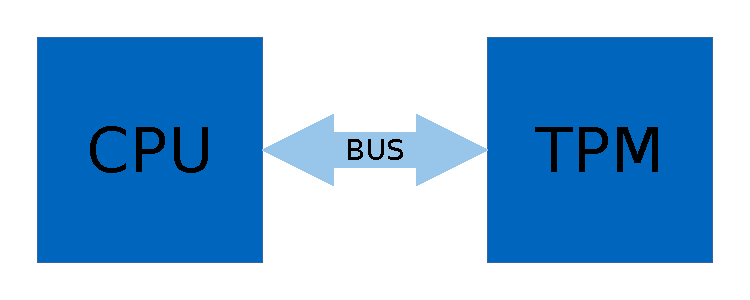
\includegraphics[width=\linewidth]{figures/dTPM.pdf}
      \caption{Discrete TPM} \label{fig:dtpm}
    \end{subfigure}%
    \hspace*{\fill}   % maximize separation between the subfigures
    \begin{subfigure}{0.49\textwidth}
      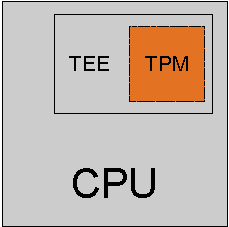
\includegraphics[width=\linewidth]{figures/fTPM.pdf}
      \caption{Firmware TPM} \label{fig:ftpm}
    \end{subfigure}%

    \begin{subfigure}{0.49\textwidth}
      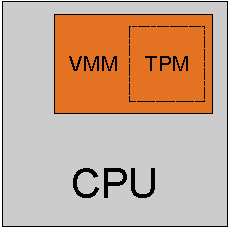
\includegraphics[width=\linewidth]{figures/vTPM.pdf}
      \caption{Virtual TPM} \label{fig:vtpm}
    \end{subfigure}%
  
  \caption{Schematic illustration of the different TPM types. Blue: Hardware, Orange: Software.} \label{fig:tpm_types}
  \end{figure}

There are three types of TPMs. They all offer the same functionality, but with different security guarantees and performance characteristics.

\subsection{Discrete TPM}

This is the classical form of a TPM. It is a dedicated piece of hardware, connected to the CPU via a bus. It is designed and manufactured to be highly temper-resistant against hardware attacks.
The TPM specifications \cite{tpm, tcgPcClient} do not demand a specific bus system, however, they define the interfaces between the TPM and the following bus systems: LPC, I\textsuperscript{2}C, and SPI.

The well-known 'TPM Reset Attack' was independently described in \cite{kauerBernhard,sparks2007}. It requires minimal hardware, precisely only a wire connecting the reset line of the LPC bus \cite{lpc} to ground. This results in a reset signal for the TPM, yielding predictable values for the \ac{PCR} registers, i.e., 0. This allows an attacker to replay the measurement log of a benign boot process to achieve valid \ac{PCR} values, even though a modified chain has been booted.
Since TPM 1.2, TCG provides a mitigation specification for this reset attack \cite{tcgResetFix}, requiring the BIOS to overwrite sensitive data after each unexpected reset, preventing an attacker to gain a valid measurement log.
% TODO: That's claimed by Winter2013 but that the mitigation works because the attacker cannot gain a valid measurement log is from me. But is measurement log really sensitive? Otherwise I'm not sure how the mitigation prevents the attack, since the spec only changes the behavior of the platform on reset, not the TPM on reset. And with the upper described attack, only the TPM is reset.
However, this mitigation is still vulnerable to cold boot attacks \cite{Halderman2009, Winter2013}.

Winter and Dietrich \cite{Winter2013} demonstrate a bus modification attack at TPMs integrated with the LPC bus or the I\textsuperscript{2}C bus.
Their approach, labeled 'Active LPC frame hijacking', allows them to "lift" commands to a higher locality than the one they were originally sent with. This allows them to evolve the 'TPM Reset attack' from being only usable for S-RTM, to also D-RTM systems.
They also introduce a new approach of circumventing the TPM's measurement feature. Instead of resetting the TPM as previously described \cite{kauerBernhard,sparks2007}, they reset the main device, i.e., the users' device like a desktop PC while preventing the TPM from receiving the reset signal. This keeps the state of the TPM, e.g., the valid \ac{PCR} values of the previous boot procedure, and the attacker can hijack the boot procedure triggered by the platform's reset and boot a malicious operating system or firmware, while the TPM still stores the old and valid PCRs. While its conceptually easier since the attacker does not need to know the measurement log since the valid \ac{PCR} values are already in-place, it requires active manipulation of bus transmissions to shield the TPM from the reset signal.

A passive sniffing attack is shown in \cite{Kursawe2005AnalyzingTP}. It is applicable to TPM 1.1 connected to an LPC bus. They observed that the data of some operations like unsealing are transmitted via the bus in plain text. Since TPM 1.2, however, the modules no longer send sensitive data unencrypted \cite{Winter2013}.

That invasive hardware attacks against dTPMs are possible was already proven by Tarnovsky in 2010 \cite{tarnovsky}. However, this requires a lot of time, knowledge and resources, i.e., hardware and money.


\subsection{Firmware TPM}

As seen in the previous section, the bus between the CPU and a TPM is the biggest attack vector. An fTPM circumvents this by being directly executed within the CPU, revealing no easily accessible bus.

\subsection{Virtual TPM}

% Confidential Computing approaches (Fraunhofer paper), our solution could be a use-case for that

% Provided by hypervisor (not necessarily, I read a paper which does not need to trust hypervisor. Don't remember what provides it.)


\section{Secure Boot and Measured Boot}

Secure boot is a concept of UEFI doing local attestation of components directly at boot-time. Based on signatures of next-to-boot components. It cancels the boot process as soon as deviations are detected. Binaries of components are first signed and then, deployed universally. Hence, binaries are not bound to the platform and can be considered portable in this context.

Measured Boot is a concept that is often implemented in interplay with a TPM. Measured Boot allows remote attestation to a later time. Uses sealing functionality of TPMs, therefore, bound to the exact platform.

Both technologies are often used in conjunction.

% !TeX root = ../main.tex
% Add the above to each chapter to make compiling the PDF easier in some editors.

\chapter{Related Work}\label{chapter:related_work}

In this chapter we provide a collection of scientific work that relates to this thesis.
For each, we provide a brief overview and how they are connected to our work.

\section{Attacks on TPMs}

Generally, attacks on \acp{TPM} target one of two goals.
Either to decouple the host system's actual state and the state measured by the \ac{TPM}, or to reveal secrets stored on the TPM\@.


% Attacks on \acp{dTPM} are relevant as they motivate \acp{fTPM}.
% We also introduce attacks on \acp{fTPM} to show that updates and measuring the exact version of them are important to understand which known vulnerabilities are patched and which are not.

% \subsection{\Acl{dTPM}}

\paragraph{\Acl{dTPM}}

The `TPM Reset Attack' on TPM~1.1 is described independently in~\cite{kauerBernhard,sparks2007}, whereby the state of the host computer and the TPM are decoupled.
It requires minimal hardware, precisely only a wire connecting the reset line of the LPC bus~\cite{lpc} to ground.
The TPM understands this as a reset signal, yielding predictable values for the \ac{PCR} registers.
This allows an attacker to perform a boot process with malicious components, later resetting the \ac{PCR} values to a known value with the reset attack, and then replay the measurements of a benign boot process.
This not only spoofs the attestation process, but also allows the attacker to access secrets stored on the TPM, which is sealed to the benign state of the host machine.
\Ac{TCG} mitigated this problem by introducing localities with TPM~1.2 which restrict the extension of specific \acp{PCR} to special hardware modes that are no longer accessible in the later boot process~\cite{tpmResetMitigation}.

Winter and Dietrich~\cite{Winter2013} circumvent this counter measurement with an attack on \acp{dTPM} integrated with the LPC bus or the I\textsuperscript{2}C bus.
Their approach---labeled `Active LPC frame hijacking'---allows them to ``lift'' commands to a higher locality than the one they were originally sent with.
% This allows them to evolve the `TPM Reset attack' from being only usable for \ac{SRTM}, to also \ac{DRTM} systems.
They also introduce a new approach to disconnect the \ac{TPM}'s measured state and the systems actual state.
Vice versa to the `TPM Reset Attack', they reset the main device, e.g., a personal computer, while preventing the TPM from receiving the reset signal.
This keeps the benign measurements stored by the TPM, while the attacker can compromise the newly booting system without being measured.
% While this is conceptually easier since the attacker does not need to know the measurement log since the benign \ac{PCR} values are already in-place, 
However, it requires active manipulation of bus transmissions to shield the \ac{TPM} from the reset signal.
The original work is from 2013 and therefore focuses on TPM~1.2.
Despite only having access to TPM~2.0 emulators in 2015, Winter mentions in his master's thesis that initial tests indicate that these attacks also apply to TPM~2.0.
To the best of our knowledge, this is the only statement done about these attacks for TPM~2.0.


% A passive sniffing attack is shown in~\cite{Kursawe2005AnalyzingTP}.
% It is applicable to TPM~1.1 connected to an LPC bus.
% They observed that the data of some operations like unsealing are transmitted via the bus in plaintext.
% Since TPM~1.2 the modules no longer send sensitive data unencrypted~\cite{Winter2013}.

% That invasive hardware attacks against \acp{dTPM} are possible was already shown by Tarnovsky in 2010~\cite{tarnovsky}.
% Nevertheless, this requires a lot of time, knowledge and resources, i.e., hardware and money.

% \subsection{\Acl{fTPM}}
\paragraph{\Acl{fTPM}}

As seen in the previous section, the bus between the CPU and a \ac{dTPM} is a typical attack vector throughout their history.
An \ac{fTPM} circumvents this by being directly executed by the CPU within a \ac{TEE}, revealing no easily accessible bus.

Despite that, there are also attacks against \acp{fTPM}.
Moghimi et al.~\cite{Moghimi2019} demonstrate a time-based side-channel attack.
It applies to Intel's \ac{fTPM} before the corresponding software patch in November 2019, and allows an attacker to recover 256-bit private keys for ECDSA and ECSchnorr signatures.
% STM published a solution, but this involves a hardware update and not just a software update.

Seunghun Han et al.~\cite{aBadDream} report two attacks on \acp{TPM} to reset the PCR registers.
The first targets a gray area in the power management section of the TPM~2.0 specification.
If the host platform goes into sleep mode, it can send a command to the TPM demanding it to store its current state including its PCRs in its non-volatile random access memory.
When the host platform wakes up again, it can request that the saved state be restored with a corresponding command.
Nonetheless, the specification lacks a concrete description of the behavior if the TPM has not saved any state before going to sleep, but still receives the command to restore its saved state when waking up.
It merely states that the TPM implementation is expected ``to take corrective action.''
Hence, some implementations simply reset the TPM which resets the \acp{PCR} as well, which also applies to the latest version of the TPM specification at the time of writing~\cite{tpm20}.
Their second attack targets an \ac{fTPM} running with Intel's Trusted Execution Technology.
They exploit that some mutable function pointers are not measured in its measuring boot environment.

Jacob et al.~\cite{Jacob2023} target proprietary AMD fTPMs by attacking their \ac{TEE}, namely the AMD Secure Processor~(AMD-SP).
Thereby, they can expose the full internal state of the \ac{fTPM} bypassing any authentication mechanisms.
To do so, they leak the secret key from the BIOS flash chip which is used to derive the encryption and signature keys for the \acp{fTPM} non-volatile data.
They achieve this by using a voltage fault injection that bypasses the authenticity check in the host's boot process and allows them to boot their own firmware component that leaks the required information.

Cohen from the Google Cloud Security team also targets AMD's fTPM running with the AMD-SP~\cite{cohen}.
They store a maliciously crafted payload---a certificate---on the \ac{fTPM} and trigger a function with a stack-based overflow error that accesses this payload, giving them full control over the program counter.
According to the author, this bug is limited to vendors that diverge from the \ac{TPM} specification, as this issue does not appear in \ac{TCG}'s reference code.

These attacks on \acp{fTPM} show that they need to be updatable to respond to the disclosure of future vulnerabilities.
They should also be measured to understand which known vulnerabilities are patched and which are not.

\section{Hardening of TPMs}

In the following, we describe defense mechanisms for fTPMs that can be seen as complementary to our approach.
They all have in common that they offer no way for a third party to ensure that the hardened fTPM is actually running on the device under test, which is exactly what our work aims to cover.

\subsection{Firmware TPMs}

One approach is to formally verify the code of fTPMs towards specific security properties.
Mukhamedov et al.~\cite{Mukhamedov2013} write portions of the TPM~1.2 code in a functional programming language---namely F\texttt{\#}---that enables automatic verification.

Raj et al.~\cite{Raj2015} call for hardware entropy for a secure \ac{fTPM} implementation, but do not elaborate on how this can be achieved.
Kim and Kim~\cite{Kim2019} propose an abstraction layer on top of an \ac{fTPM} and a \ac{dTPM}---the hybrid TPM~(hTPM), which enables switching between the hardware and software module as required.
They aim to combine their advantages, e.g., by making the dTPM the source for the hardware entropy of the fTPM\@.
In addition, the hTPM performs significantly better in software mode than in hardware mode due to the use of modern CPU features.
But for all that this comes at the cost of increasing complexity.

In contrast, Gross et al.~\cite{Gross2021} propose backing an \ac{fTPM} with hardware without requiring a \ac{dTPM}.
For that, they provide cryptographic and entropy support through hardware.
This inherits the downsides of \acp{fTPM} which are not related to a lack of hardware, but to the nature of software.
For example, their \ac{fTPM} is still started later in the boot chain than a \ac{dTPM}, which is not the case for an hTPM\@.
Despite that, it is easier to update than hTPM since the lack of a dTPM, and the overall design is simpler.

\subsection{Virtual TPMs}

% Due to the increasing popularity of cloud computing, the research of vTPMs focuses less on specific attacks, and more on reducing the trusted computing base, i.e., privacy-focused.
The initially proposed design of virtual \acp{TPM} requires the operating system and the hypervisor to be trusted~\cite{268868}.

Wang et al.~\cite{Wang2019} bring the vTPM into the \ac{TEE}, namely Intel SGX, essentially creating an fTPM and vTPM hybrid.
They launch each vTPM in a private hardware-protected enclave.
This reduces the required trust into to the individual enclaves and SGX itself, enabling the host operating system and hypervisor to be untrusted.

Pecholt and Wessel~\cite{Pecholt2022} describe a design named CoCoTPM where the hypervisor and the host's operating system do not need to be trusted as well.
This is realized by establishing an integrity-protected secure channel with end-to-end encryption between the driver in the VM and the software TPM on the host.

Stateless ephemeral vTPMs~\cite{Narayanan2023} eliminate the need of manually establishing a secure channel by leveraging the confidential VM memory encryption provided by AMD's SEV-SNP, a variant of AMD secure encrypted virtualization~(SEV) technology.
Ephemeral vTPMs support the remote attestation of virtual machines.
On the other hand, they intentionally do not support persistent storage to preclude exfiltration attacks on the TPM's data-at-rest, which has the disadvantage that persistent keys or nonvolatile indexes cannot be stored.

\section{Remote attestation schemes}

% Other defense concepts

% Linux attested with DICE directly instead of TPM?
% Probable disadvantage: not TPMs common interfaces
% and DICE certificate chain size grows linearly, PCR register size is fixed. However, event log also grows linearly, but less data (less information, but less storage overhead)

% https://www.eurecom.fr/fr/publication/3536/download/rs-publi-3536.pdf
The SMART attestation mechanism proposed by Defrawy et al.~\cite{EURECOM+3536} establishes a \ac{DRTM}.
Since their overall approach is similar to \ac{DICE}, they only hardware requirement is a ROM containing a key (corresponding to DICE's \ac{UDS}), and that can only be accessed by SMART\@.
Their secret key is directly used to sign attestation data, while for \ac{DICE} the \ac{UDS} acts as entropy to derive individual secrets from for each firmware component.
SMART thus provides a \ac{DRTM} in contrast to the \ac{SRTM} provided by \ac{DICE} enabling the remote attestation of an \ac{fTPM}.
However, it does not allow data to be bound to the identity of a firmware component.

\ac{TCG} offers an adaption of \ac{DICE} with symmetric cryptography which conducts implicit attestation~\cite{dice-symmetric-arch}.
There, the final symmetric key---also called alias key here---derived from the compound identity of the whole firmware and its UDS represent the prover's identity, without propagating the individual identities of each firmware layer like the \acp{TCI} do.
If this alias key is leaked, trust into the system breaks unrecoverable since the same key is generated on each boot.
DICE+ proposed by Jia et al.~\cite{Jia2020} solves this by equipping the prover with a monotonic counter, which is incremented on each reboot.
This counter influences the alias key, which consequently alters the attestation result derived from it after each reboot as well.
The verifier can calculate the expected attestation data by combining the used counter value, the UDS, and the expected firmware identity.
DICE+ assumes that there is only a single verifier who knows the received values of all previously conducted remote attestations, and can therefore detect replay attacks.
The verifier and the prover must have shared secrets due to the nature of attestation based on symmetric cryptography.
DICE+ shares the prover's UDS and also the initial monotonic counter with the verifier during the prover's provisioning in an out-of-band manner.
While their approach is practical for low-end devices that are not capable of asymmetric cryptography, we are targeting machines with a processor with a \ac{TEE}, which implies a certain amount of computation power.
We also do not want to require pre-shared secrets between the verifier and the prover.
In addition, the TPM's infrastructure demands asymmetric cryptography for signing the EK certificate, and the monotonic counter would change the TPM's identity on each reboot, effectively hindering the binding of the fTPM's data to its identity.
Hence, we use DICE with asymmetric cryptography instead.

% They claim it is implicit, but I believe they have another understanding of implicit and explicit as what I use in this thesis (the one from the DICE spec). So I just leave it, as it is only confusing and not of great importance.
Bravi, Sisinni, and Lioy~\cite{Bravi2023} propose an attestation system with DICE for IoT devices running with the RISC-V ISA without TEE\@.
While we combine DICE with the TPM infrastructure, they combine it with the Manufacturer Usage Description (MUD).
MUD allows a device to signal to the network what kind of access and network functionality it requires for further access control~\cite{Lear2019}.
It also explains how DICE can be implemented with the novel RISC-V technology Physical Memory Protection~(PMP).
Their design is orthogonal to ours, and they are compatible.
This is because we are not limited to a specific DICE implementation and their support for MUD is integrated via an X.509 certificate extension that can trivially be added to our system as well.

\section{DICE implementation}

Jäger, Petri, and Fuchs~\cite{Jaeger2017} describe how the remote attestation procedure described in the DICE specification can be put into practice by discussing implementation options.
Thereby they complement our work by evaluating how to implement \ac{DICE}\@.
Jäger and Petri continue their work later~\cite{Jaeger2020} because they observed a limitation in their initial implementation, allowing to jump into \ac{DICE} code possibly leaking the \ac{UDS}.
Lorych and Jäger carried on exploring the design space of DICE~\cite{Lorych2022} later on.
As with SMART, the goal of all these publications is not to attest an \ac{fTPM} and therefore do not describe how to combine the infrastructure of DICE and \acp{fTPM}.

Just as we presented a paper proposing a formally verified \ac{fTPM} implementation, Tao et al.~\cite{272306} propose a formally verified \ac{DICE} implementation called DICE\( ^* \).
They focus on the software side of the first DICE layer and are agnostic to the actual hardware used.
Therefore, it can be used together with the hardware designs from the previously listed works.

% TEE attestation

% M{\'{e}}n{\'{e}}trey et al.~\cite{Menetrey2022} discuss attestation mechanisms for \acp{TEE}.
% Our \ac{fTPM} is also running in a \ac{TEE}, and can thereby be attested with this approach.
% However, it assumes that the entire TEE is trusted


% Attacks which we would avoid (e.g., exchange/spoof EKcert)


% https://dl.acm.org/doi/pdf/10.1145/3600160.3600171
% This requires trusting the measurement root of trust (there TPM, AMD SEV-SNP or Arm PSA Attestation Token), but also need to trust the operator to provide benign reference values.
% Or not if the operator of the trust anchor is the same as the operator of the device. Or the trust anchor and the reference values root in the operator. Operator needs to sign (and beforehand verify) not only the trust anchor, but also reference values (high burden).
% The paper also only mentions hardware trust anchors, no fTPMs. Could be used in conjunction. I believe our cert chain up to the fTPM would need to be provided within the Attestation Report, but system independent, i.e., would need to be independent of the concrete technology (here DICE). Not sure if that's possible.

% https://www.amd.com/en/processors/amd-secure-encrypted-virtualization
% For virtual machines
% Auch https://arxiv.org/pdf/2204.06790.pdf
% 3.5

% https://ieeexplore.ieee.org/abstract/document/9292371

% https://netsec.ethz.ch/publications/papers/mccune_parno_perrig_reiter_isozaki_eurosys08.pdf

% !TeX root = ../main.tex
% Add the above to each chapter to make compiling the PDF easier in some editors.

\chapter{Methodology}\label{chapter:methodology}

\section{Terminology}\label{sec:terminology}

Before we dive into technical explanations, we want to clear some potential terminology confusion.

In the original DICE release from Microsoft~\cite{England2016}, the identifier of a component is called the \ac{FWID}.
The \ac{TCG} consortium later renamed it \ac{TCI}.
We believe this is to emphasize that the TCI does not necessarily have to be the hash of a firmware binary, but could also be, for example, the embedded ID of a hardware component.
However, \ac{TCG} has not fully adopted this terminology renaming.
Their DICE Attestation Architecture~\cite{TCGAttestation2021} defines an X.509 extension that contains the \acp{TCI}.
They continue to be referred to as \acp{FWID} in the machine-readable formal definition of this extension, while everywhere else they are referred to as \acp{TCI}.
In personal correspondence with \ac{TCG}, we have learned that this is due to backwards compatibility.
The old term \ac{FWID} is retained whenever it is used in something that is alive in the long term, like formal definitions, and the new term \ac{TCI} in assets that can be updated more quickly, such as the specification text.
Therefore, we will use the term \ac{TCI} in this theoretical chapter, and in the implementation chapter (\autoref{chapter:implementation}) we will use the term \ac{FWID}, just as it is common practice at the \ac{TCG}\@.
This ensures that the explanation of our implementation better matches the actual code, where \ac{FWID} is the term as it is used by automatically generated code.

Occasionally, the name of an asymmetric key is suffixed with `priv', `pub' or `cert' to designate the private part, the public part, or the certificate, respectively.
For example, EKpriv refers to the private portion of EK\@.
And EKcert corresponds to the certificate with EKpub as its subject key.

% Prover/Verifier (in many earlier papers) vs. Attester/Verifier/Relying Party (RFC)


\section{Architectural overview}\label{sec:arch_overview}

\begin{figure}[htpb]
  \centering
  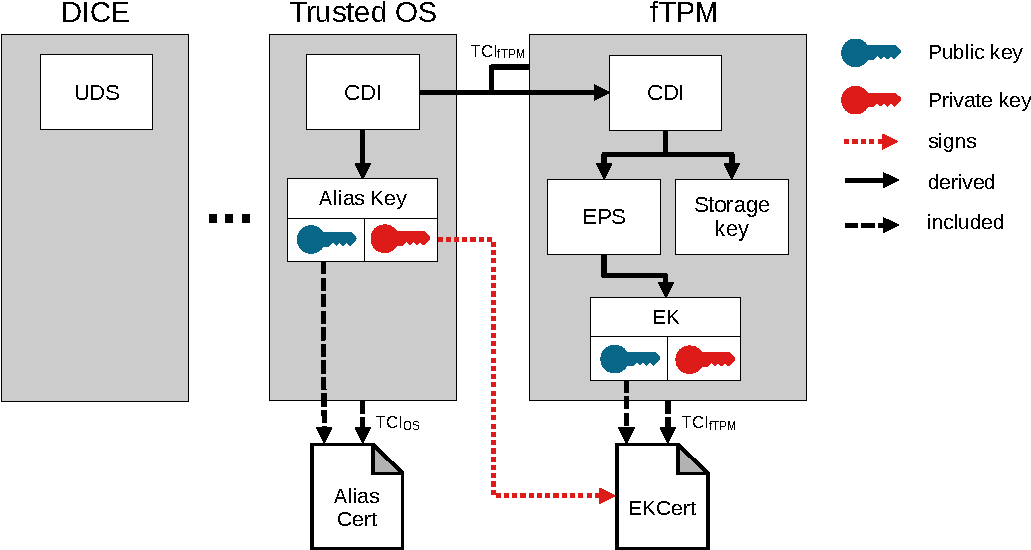
\includegraphics[width=1\linewidth]{figures/architecture.pdf}
  \caption{The architecture of our system.} \label{fig:architecture}
\end{figure}


The architecture of our proposed and later implemented system is illustrated in \autoref{fig:architecture}.
As you might notice, it is similar to our overview picture of \ac{DICE} (\autoref{fig:dice-layers}).
This is to be expected, since our system leverages \ac{DICE} as our \ac{SRTM}.
% TODO: Rework depending on when DRTM/SRTM are introduced
Static in this context means that it uses the trusted state that a device has at the always same point in time, here after switching on, for further measurements.
This is in contrast to a \ac{DRTM}, which is able to do this at any time, e.g., Intel SGX\@.

The boot process continues from here in the usual \ac{DICE} manner until the firmware TPM is reached.
The component that measures the \ac{fTPM} is usually the trusted operating system running in EL1 in the secure world, as seen in \autoref{fig:arm_trustzone_arch}.
Like any other \ac{DICE} component, the \ac{fTPM} receives its secret \ac{CDI} from its predecessor layer.
Recall that the \ac{CDI} is tied to the identity of the \ac{fTPM} including the entire underlying firmware stack and the \ac{UDS}\@.
We derive two values from the \ac{CDI}\@.

\subsection{Storage key}

% Storage Key generation

While the trusted OS within the \ac{TEE} might already encrypt data before it is sent to the storage device, this only binds the data to the \ac{TEE}, but not the identity to the \ac{fTPM}.
For this purpose, we first derive a storage key from the \ac{CDI}.
This is a symmetric encryption key that is used to encrypt the \ac{fTPM} storage space in RAM before it is written to a persistent storage space such as a hard disk drive~(HDD).
At no time does the HDD see plaintext data (\autoref{fig:storage-encryption}).
As the storage key is derived from the \ac{CDI}, the storage data is only accessible to the \ac{fTPM} with the exact identity with which it was generated.
For example, its identity changes due to a \ac{TPM} modification or an update of a previous firmware component, which results in a full manufacturer reset of the fTPM\@.
This enables the property that an \ac{fTPM} storage must never be accessible to another \ac{TPM}\@.

\begin{figure}[htpb]
  \centering
  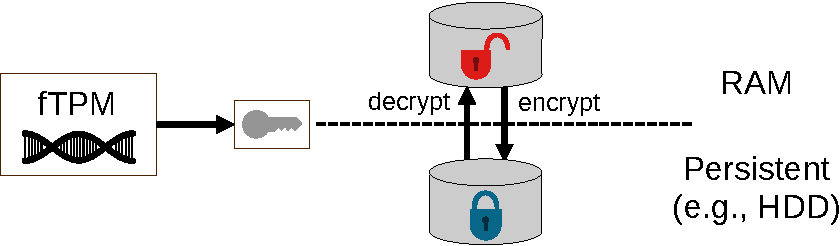
\includegraphics[width=0.8\linewidth]{figures/storage-encryption.pdf}
  \caption{The fTPMs' storage is protected by a key derived from its identity.} \label{fig:storage-encryption}
\end{figure}


An attacker could thereby easily trigger a data loss.
This must be avoided by integrating good-practices with working with a \ac{TPM}, which includes having secrets stored also elsewhere.
Microsoft recommends backing up all secrets stored on the \ac{TPM} before clearing it~\cite{MicrosoftClearRecommendations}, what can be generalized to the backup of the fTPM data in all cases where data loss causes serious damage.

% For pure data or fTPM rollback: RPMB reduces possible attackers to components in the TEE. No entire protection.
% But for data protection by downgrading the fTPM: Our solution is more secure than only using RPMB, see paragraph below. In short, we do not need to trust entire software stack in TEE.

Establishing the storage key also prevents an attacker from accessing an fTPM's data by downgrading the fTPM\@.
For example, if an attacker wants to access data stored in a particular fTPM and can exploit a vulnerability of an earlier version of that fTPM, it is not possible to replace the fTPM with its old version, as neither the attacker nor the fTPM itself will be able to decrypt the previous data.

However, it does not protect against the isolated downgrade of the fTPM itself or solely its data.
When the fTPM is downgraded, as previously described, the data is reset.
Nevertheless, new data generated by the downgraded TPM might still be leakable by vulnerabilities of the downgraded fTPM\@.
Our storage key also does not protect the fTPM data from a rollback attack, i.e., the freshness of the fTPM data is not guaranteed.
This attack can be attractive for malicious actors to reset the try count of PINs to work around the lockout mechanism of the TPM\@.
Another example is to restore the data wherein a secret was stored, however, not yet protected by a PIN\@.
% A malicious actor requires the TPM to decrypt the data, as it is encrypted.
The protection against the rollback of fTPM data or the fTPM itself can be achieved by storing them in a Replay Protected Memory Block~(RPMB) partition~\cite{eMMC, UFS}.
For this reason, an RPMB partition is part of Microsoft's hardware requirements for a firmware TPM~\cite{Raj2015}.

Only the TEE can write to the RPMB (authenticated write).
And the TEE can ensure that received data really originates from the RPMB (authenticated read).
Each command is unique due to a nonce (for read operations) or a write counter (for write operations), which prevents replay attacks.
The secure channel to the RPMB is established by a secret key shared between the TEE and the RPMB\@.
Hence, every component within the TEE can arbitrarily access and modify the data on the RPMB, and must therefore be trusted.
This is different to our approach with the storage key, whereby we bind the access to the data to the identity of the fTPM, i.e., we trust only the identity of the fTPM instead of the entire TEE\@.
In other words, we seal the data of the fTPM with the identity of the fTPM instead of allowing the entire TEE to access the data at any time.
However, RPMB and our storage key are orthogonal and can be used in conjunction.

% , as each component in the TEE can read from or write to the RPMB partition arbitrarily.
% This is independent of the component's identities.
% In our approach with the storage key, the fTPM does not have to trust its preceding components, because as soon as one of them changes, the fTPM itself no longer has access to the data.

% Indeed, the fTPM itself can also be stored in a RPMB partition, which builds another rollback protection aside of our approach with the storage key.
% However, this protects the data on different levels.
% The encryption with our storage key introduces confidentiality and integrity of the fTPM's data sealed to the identity of the fTPM\@.
% RPMB protects the data's confidentiality, integrity and freshness from access outside the TEE, assuming the RPMB is only accessible from the TEE, which is the typical design.
% Hence, while the RPMB protects additionally freshness, we bind our security guarantees tighter to the exact identity of the fTPM instead of merely to the specific TEE\@.

% So, our mechanism additionally protects data-at-rest, while the data-at-use is protected by the TEE's secure memory, i.e., the memory isolation from the normal world.

\subsection{EPS and EK}

% EPS Generation

Then, the \ac{EPS} is generated based on the \ac{CDI}\@.
It is the seed that is used to generate the primary \ac{EK}.
A primary key in the sense of the TPM means that it has no parent key, but a parent seed, here the \ac{EPS}\@.
The indirection of generating the \ac{EK} from the \ac{EPS} via the \ac{CDI} instead of generating it directly from the \ac{CDI} is introduced because the code of fTPMs can be hardcoded to use the \ac{EPS} during \ac{EK} generation.
And we want our system to require as few modifications to TPM code as possible.
The \ac{CDI} must also be removed from memory as quickly as possible to reduce the time frame in which leaks are possible, but the \ac{EPS} must be accessible to the \ac{fTPM} throughout its entire runtime.
It is therefore good practice to extract long-term secrets from the short-term secret \ac{CDI} and then quickly delete the \ac{CDI} from memory.

% Device identification

The \ac{EK} of a \ac{dTPM} represents the long-term identity of its host device as long as the \ac{TPM} is not soldered or plugged away.
Our \ac{EK} does not do this because an \ac{fTPM} is software-based and changes every time the \ac{fTPM} or the underlying firmware is modified, without the host device changing.
Instead, we use the DICE for this, which is hardware-based.
Its DeviceID key, as the name suggests, represents the device identity.
Note that the DeviceID contains the identity of layer 0 of the boot chain, i.e., the first mutable code.
This can also be seen in \autoref{eq:dice_deviceID}.
For this reason, the DICE specification suggests keeping the first mutable code as small as possible so that it remains constant throughout the life of the device~\cite{dice-layering-arch}.

% EK is a signing key

By default, the \ac{EK} is a restricted encryption key.
It is not used for signing by default because the resulting signatures may reveal the TPM's identity.
We deviate from that by creating the \ac{EK} as a restricted signing key.
While this breaks privacy of the prover, it has the advantage of not requiring a third party \ac{CA}\@.
More details and an extension to our system introducing privacy is provided in \autoref{sec:privacy}.

\section{The identity of a firmware TPM}

DICE offers two identities for each component---the TCI and the CDI\@.
As shown in \autoref{eq:dice_cdi}, the CDI of a component changes when (i) the identity of the hardware changes, i.e., the \ac{UDS}, (ii) the identity of a preceding component changes, or (iii) the component itself changes.
In contrast, the TCI is the identity of a single component, considered in isolation, usually the hash of its binary, i.e., only for case (iii).
% It only changes when the component itself is changed, regardless of the hardware or preceding components.
So, while a CDI should be statistically unique since it is derived from a \ac{UDS} with this property, a given TCI can be found on many devices if they contain exactly the same software component.
Note that a component's TCI is part of its CDI, as shown in \autoref{fig:identities}.

\begin{figure}[htpb]
  \centering
  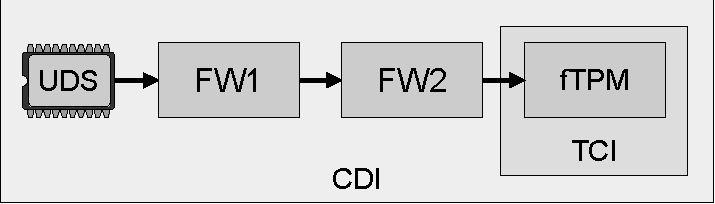
\includegraphics[width=0.6\linewidth]{figures/identities.pdf}
  \caption{Visualizing the difference between the CDI and the TCI from the perspective of an fTPM component. The identity of the hardware is provided in the form of the UDS.} \label{fig:identities}
\end{figure}


Hence, we decided to derive the identity of an fTPM, i.e., its \ac{EK}, ultimately from the CDI\@.
This binds the identity of the fTPM to any security-relevant component preceding it.
The rationale for this is that once a previous component has changed, it is unknown whether it has gone into a benign or malicious state.
And if it is malicious, it could change the firmware TPM and thereby access its sensitive material such as private keys.
Although this is later recognized by the verifier during remote attestation, sensitive data could still be leaked.
If the identity of the firmware TPM is extended to everything prior to the fTPM, its data is no longer accessible as soon as something preceding it changes.
This is due to the derivation of the storage key from the CDI\@.
And this behavior should also be reflected in the EK, so that the storage key and the EK should always change together or not change at all.

The TPM's storage cannot be part of its identity as it changes during runtime after each data write, e.g., storing an arbitrary key.
This is a problem because DICE only runs during the boot time in which the identity of the fTPM is measured.
The identity of the fTPM must not change afterwards, otherwise the identity reported by DICE and the actual identity of the fTPM would be inconsistent.
We also do not want to restrict the permissible values of the working data of an fTPM, which makes its measurement as part of the TCI pointless.

% Depending on the point of view, there are two identities of an fTPM, as shown in \autoref{fig:identities}.
% There is the identity of the fTPM measured by DICE, which consists of the hash of the binary and the component configurations as for all DICE components, as shown in \autoref{fig:ftpm-identity}.
% This identity is referred to as the TCI.
% Compilation flags are not part of these configurations, as they are embedded in the final binary and are therefore automatically measured as part of the measurement of the binary.
% Of more interest are the configurations that are not part of the binary.
% They are usually provided in well-known formats such as \texttt{json} or \texttt{xml}.
% However, Microsoft's fTPM reference implementation does not contain such configurations, which simplifies the TCI generation of our fTPM by limiting it to the measurement of the fTPM binary data.
% The TPM's storage cannot be part of its identity as it changes during runtime after each data write, e.g., storing an arbitrary key.
% This is a problem because DICE only runs during the boot time in which the identity of the fTPM is measured.
% The identity of the fTPM must not change afterwards, otherwise the consistency of the identity transmitted by DICE and the actual identity of the fTPM would differ.
% We also do not want to restrict the permissible values of the working data of an fTPM.
% In summary, the CDI keeps being updated from layer to layer, the TCI is calculated for each layer individually.
% Then, there is also the identity of the fTPM in the TPM context, which is represented by its EK.
% This identity is not only bound to the binary and the configuration of the fTPM, but also the entire underlying firmware stack.
% We derive the EK from the TPMs CDI, which is derived of the measurements of all preceding firmware components and the TPM's TCI, see \autoref{eq:dice_cdi}.

% \begin{figure}[htpb]
  \centering
  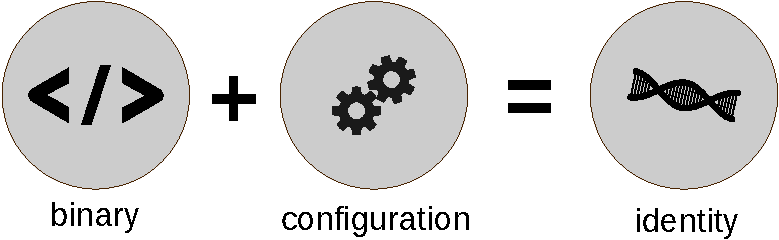
\includegraphics[width=0.6\linewidth]{figures/ftpm-identity.pdf}
  \caption{The accumulation of the binary and its configuration to its identity.} \label{fig:ftpm-identity}
\end{figure}


% Configurations required
% Does contain whole firmware stack?
% Data cannot be considered, since changes during runtime, not represented by DICE which only happens at boot-time
% What happens if identity changed? -> Data not accessible, in essence, fTPM fully reset
% https://trustedfirmware-a.readthedocs.io/en/latest/design_documents/measured_boot.html#critical-data

% \section{Provisioning process}

% To summarize, attestation key provisioning must ensure that only valid attestation key material is established in Attesters [RFC 9334]

\section{Attestation process}\label{sec:attestation_process}

% Check also for revocation of manufacturer cert

% We use explicit attestation. See DICE Layering Spec 7.2
% See 8.1.1.2 for an example about implicit attestation
% Implicit attestation would require to know all resulting public keys in EKcert, which would require that we booted it up in a controlled manner beforehand and stored the resulting code.
We use an explicit attestation procedure.
This makes it sufficient for the verifier to know its trusted TCIs, whereas implicit attestation would require a database of trusted Alias public keys representing a trusted component.
And since each Alias public key is device unique, as it roots in the device's unique \ac{UDS}, the verifier would need to know all alias public keys for each component on every device declared trustworthy, which we consider unrealistic.
Also, this would be a hindrance as the verifier should be able to establish trust into an unknown device by trusting the DICE manufacturer, and knowing the identities of trustworthy firmware.

% Secure channel must be established by requiring communication with the private key corresponding to the public key in the EKcert.
% This allows a verifier to validate that the prover is in posession of the private key, and hence, the included identities in the certificate chain are trustworthy.

\subsection{Verifier establishes trust to the prover's fTPM}\label{subsec:trust_prover_tpm}

% It is exactly the purpose of our system to make this possible for the verifier.
First, the verifier retrieves the DICE certificate chain generated by our solution from the prover.
After verifying that the signatures of the certificate chain are valid, the verifier checks whether the DICE implementation is trustworthy by knowing its manufacturer.
This also involves checking if the DeviceID certificate issued by the manufacturer was revoked.
Such an event might occur if the security of an old DICE implementation is broken, and the manufacturer wants to reflect this.

At this point, the verifier must traverse the certificate chain starting from the root and verify whether each component represented by a certificate is trusted, by checking the embedded TCI\@.
An untrusted component must be assumed to lie about its conducted measurements.
For example, it can modify the subsequent component without reflecting this in the measurement of the TCI\@.
Consequently, as soon as a component is untrusted, all subsequent components have to be considered untrusted as well.
This behavior is also represented mathematically in \autoref{eq:dice_attestation}.
Therefore, trusting the fTPM requires to trust all underlying firmware components.
\begin{equation}
    \label{eq:dice_attestation}
    C_{i, \, trusted} \, \coloneqq \, \bigwedge_{k=0}^{i} trusted(C_{k})
\end{equation}

% \subsubsection{Example security policies for a component}

The \(trusted\) function of \autoref{eq:dice_attestation} checks the information provided by a certificate~\(C\) against security policies defined by the verifier.
In the following, we would like to present some example policies for improving comprehensibility for the reader.

\begin{itemize}
    \item We generally do not trust the component's manufacturer and therefore, do not trust the component.
    \item The component is up-to-date, and there are no known vulnerabilities and therefore, we trust the component.
    \item The component is outdated, but all updates are only functional instead of security-relevant, so we still trust it.
    \item We do not know the TCI of the component. We follow a `Deny by default' policy. Therefore, we do not trust the component.
\end{itemize}

After doing all this, the verifier can only state that ``I trust the certificate chain and the components of \emph{some} machine represented by it.''
This is due to the possibility of any actor to simply replay the certificate chain.
But we need to promote the \emph{some} to \emph{the machine I communicate with}.
This is solved in subsequent protocols where the prover is challenged to be in control of EKpriv which corresponds to the EKpub of the EK certificate.
For example, by verifiying the subsequently retrieved quote.
Although this is not explicitly part of our proposed solution, we nevertheless describe it for better understanding and provide a comprehensive explanation of the entire attestation process.

\subsection{Verifier establishes trust to the prover's quote}\label{subsec:trust_quote_from_prover}

For that, the verifier needs to know that the quote was signed with the restricted EKpriv corresponding to the EKpub in EKcert, and that the fTPM is in control of EKpriv.
The verifier also needs to trust that the fTPM did not leak EKpriv, as this would not only allow to replay a whole certificate chain, but even succeed the subsequent protocols with the leaked EKpriv.
The verifier can derive whether it considers the EKpriv of the fTPM as not leaked based on the fTPM's TCI value, as one requirement of trusting a TCI must be whether the verifier considers the component to keep its security guarantees.

To trigger the protocol, the verifier sends a nonce to the prover, which includes it in the quote request sent to the firmware TPM, i.e., \texttt{TPM2\_Quote}.
The nonce prevents replay attacks.
The verifier also needs to know that the EK is restricted.
Otherwise, a compromised prover could generate quotes representing arbitrary states which do not represent the prover's actual state.

Usually, this is ensured by manufacturers in that they only sign an EKcert for a restricted EK\@.
Of course, this cannot be applied to our solution, as our EKcert is dynamically created without a TPM manufacturer asserting specific attributes of the EK\@.
Instead, the verifier needs to derive from the fTPM's TCI embedded in the EKcert that the EK is restricted.
For the EK's attributes to be represented in the TCI, the template containing the EK's attributes must be generated in the firmware TPM's code.
This ensures that the TCI also represents the template.
% And, the verifier must only trust fTPM TCI's which have the restricted attribute of the EK baked in code.

% Alternative solution
% Template und EK an Optee OS, prüfen ob EK reproduzierbar und restricted in Template gesetzt. Nachteil: Algorithmus muss in TPM und Layer davor identisch sein, Abhängigkeit. Vermutlich muss TCI immer noch vertraut werden, dass TPM wirklich gleichen Algorithmus einsetzt. Und DICE Layer vor fTPM muss fTPM aware sein
% Downside: komlexer, n-1 muss DICE aware sein, und man transferiert das Vertrauen in das restricted Attribut eigentlich nur zu n-1 statt zu n, wie in der ersten vorgestellten Lösung.
% Aber keine Vorteile? Also erwähne ich es auch nicht, hat keinen Mehrwert

% \subsection{Does the remote attester trust the event log?}

% [Eventlog](https://www.notion.so/Eventlog-c1e76f302470468aa2064ca35ae1a577?pvs=21)

% In summary, it's reduced to the question whether the attester trusts the quote.

% Also, the event log is not a hard requirement. It just makes the attestation process more flexible and comprehensible, probably not required for my Proof of concept implementation.

\section{Combining TPM and DICE infrastructure}

The result of our DICE boot process is a certificate chain, starting with the manufacturer certificate and DeviceID certificate, and ending with the EK certificate.
In between can be an arbitrary number of Alias certificates for ``ordinary'' firmware components (see \autoref{eq:solution_cert_chain}).
\begin{equation}
\label{eq:solution_cert_chain}
Manufacturer\ Cert \rightarrow DeviceID\ Cert\ [\rightarrow Alias\ Cert]^* \rightarrow EK\ Cert
\end{equation}

% EKcert is an AliasCert

The DICE and the TPM infrastructure intersect at the \ac{EK} certificate.
From the DICE's point of view it is an alias certificate, from the TPM's point of view it is the \ac{EK} certificate.
So, this certificate needs to fulfill the requirements for an Alias certificate from the DICE specification~\cite{DICE_certs}, and the EK certificate requirements from the TPM specification~\cite{tcg-ek}.
Therefore, we need to ensure that these two specifications declare no conflicting requirements.
DICE~\cite{DICE_certs} defines the requirements for various certificate types.
Our certificate is referred to as an attestation certificate in their specification.

We only consider restrictions for the X.509 fields that are absolute requirements, i.e., declared as ``MUST'' according to RFC 2119~\cite{Bradner1997}.
In general, the EK certificate specification ``does not preclude the use of other certificate extensions.''
The alias certificate specification leaves this undefined, i.e., it makes no statement whether this is permitted or prohibited.
However, it is irrelevant for us, since the EK certificate specification does not define any own X.509 extensions.
The requirements about the certificate's validity depend on whether the measuring firmware has access to a secure real-time clock~(SRTC) containing the absolute physical time.
We assume the firmware to not having access to an SRTC, keeping the requirements low.
The restrictions of our certificate also depend on its further usage.
It is a leaf of the certificate chain.
Therefore, we do not consider requirements for a certificate representing a \ac{CA} signing further certificates.

We present the result of our compatibility study in \autoref{tab:cert_comparison}.
In summary, there are mostly no conflicts since both certificates expect the same value, both requirements can be satisfied with the same value, or only one of the certificates dictates a restriction for a specific field.

\begin{table}[htpb]
\caption[Certificate comparison]{Comparing the requirements for an Alias and \ac{EK} certificate. The upper half contains basic certificate fields, and the lower half contains certificate extensions.}\label{tab:cert_comparison}
\centering
\begin{tblr}{Q[l,m] Q[l,m] Q[l,m] Q[l,m]}
    \toprule
    Field & Alias Cert & EK Cert & Conflict \\
    \midrule
    
    {Version} & 3 & 3 & No \\
    {Subject\\ name} & {identify TCB class\\ or instance} & {uniquely identify\\ TPM or empty} & {Yes} \\
    {Issuer\\ name} & {embedded CA\\ issuing the certificate} & {entity that vouches\\ that TPM is genuine} & {No} \\
    {Subject\\Alternative\\Name} & {\( - \)} & {TPM details} & {No} \\
    {Validity\\(not before)} & {known time in recent past\\e.g., build time} & {\( - \)} & {No} \\
    {Validity\\(not after)} & {no expiration} & {no expiration} & No \\
    \midrule
    {Authority Key\\ Identifier} & {\( - \)} & {must be present} & No \\
    {Key Usage} & {not to verify signatures\\of certificates} & {verify signatures other \\ than those on certificates} & {No} \\
    {Certificate\\Policies} & {Local Attestation} & {at least one policy} & No \\
    {Basic\\Constraints} & {\( - \)} & {not a CA} & No \\
    \bottomrule
\end{tblr}
\end{table}


The only conflict is in the subject name.
An alias certificate must either identify the TCB class (general) or instance (specific), an EK certificate allows only a value uniquely identifying the TPM (specific) or empty otherwise.
So, a general term like ``fTPM'' is prohibited by the EK certificate specification, and an empty subject by the DICE specification.
The only common denominator is a unique identifier.
However, that is already part of the TCI embedded in our EK certificate.
We chose to favor the EK certificate specification here, and leave the subject name empty.
This ensures that the EK certificate is also as expected for systems that do not know our solution and do not know the TCI part of the certificate.
An empty subject names also appears to be common practice in EK certificates, as this is the subject name chosen for all EK certificates we observed.
This should not be regarded as representable, however, since the sample size is three.

The Subject Alternative Name extension is required to contain the TPM Manufacturer, model, and version by the EK certificate specification~\cite{tcg-ek}.
It is assumed that the EK certificate is generated by the manufacturer who has this knowledge about the TPM\@.
In our system, however, the DICE layer measuring the firmware TPM and ultimately generating the EK certificate does not know these values, as they are not constant and can change any time when the firmware TPM is exchanged.
One possible solution is to keep these values in the metadata of the fTPM's binary, which the preceding layer can read and embed in the certificate.
But this increases the complexity and the maintenance burden for the firmware TPM, which is usually not required since all this information (manufacturer, model, version) can be deduced from the TCI part of the certificate.
Therefore, if verifiers trust a TCI, they should also know which manufacturer, exact code and TPM specification it conforms to.

Furthermore, the TCI is more accurate and reliable because it is an exact independent measurement of the firmware TPM rather than relying on information embedded by the TPM's manufacturer.
For example, an underlying firmware component could change these details embedded in the firmware TPM to pretend that it is compliant with a newer specification with potential security updates than it actually is.
This cannot happen with the TCI, which is part of the certificate chain, as this malicious firmware component would be detected as long as it is not the first DICE layer.
To still fulfill the EK certificate specification, we suggest to use general terms.
For example, the manufacturer could be defined as ``DICE'', the model as ``FW'', and the version as TPM~2 compliant, whereby the minor version is not specified, i.e., zero.


\section{Updating the fTPM}

We consider it as critical that the \ac{fTPM} is updatable. This is due to the history of \acp{fTPM} showing vulnerabilities which have been patched consequently.
% cite... all from background probably, or ref section in Related Work
Our \ac{fTPM} can be only updated with the system shut down.
This ensures that the TCI part of the EKcert generated at boot-time does not become obsolete, in other words, keeps representing the identity of the currently running fTPM\@.
% This is due to the required out-of-band signing procedure of trusted applications before being deployed.

The code of the fTPM is replaced during an update.
The fTPM therefore retrieves a new CDI and then a new storage key.
The old data can therefore no longer be accessed, which effectively leads to a manufacturer reset.

This mechanism is common practice as this is also described in the manuals for TPM upgrades by Lenovo~\cite{LenovoTpmUpgrade} and Intel~\cite{intelTpmUpgrade}. 
It is underpinned by the importance of pausing BitLocker before upgrading a TPM due to its upcoming data loss~\cite{BitlockerTpmUpgrade}.
Thereby, BitLocker's encryption key is temporarily stored in plaintext on the hard drive, which is consequently restored on the TPM after its update.

Apart from the associated loss of data, there is no other obstacle to updating the \ac{fTPM}\@.
Updating in this sense even means replacing, e.g., with the fTPM of another manufacturer.
As it is explicitly measured, it can be replaced at will without changing the manufacturer of the \ac{DICE} or \ac{TEE}\@.

\section{Privacy}\label{sec:privacy}

First, we elaborate what reveals the identity of the device when conducting a remote attestation, and then suggest a modification to our architecture to integrate privacy.

In an ordinary remote attestation process with our system as described in \autoref{sec:attestation_process}, the verifier retrieves the certificate chain and a TPM quote.
After the root certificate, the certificate chain is continued with the DeviceID certificate, whose subject key provides the long-term identity of the device.
It then continues with alias certificates, each of which contains subject keys that represent the identity of the hardware and the firmware components executed up to that point.
The closing EK certificate of the chain contains the key representing the identity of the fTPM\@.
The quote's signature is also relevant to the prover's privacy, as it is generated with a unique EKpriv.
Consequently, all these keys have to be hidden to preserve privacy, and the signature of the quote must be generated with a key that does not represent a long-term identity.

% Therefore, the usual procedure is to create a short-lived \ac{AK} on the TPM\@.
% The verifier communicates the public part of the \ac{AK} to a third party privacy CA who ensures that the holder of the \ac{AK} is the same as the holder of the \ac{EK}, and that the \ac{EK} originates from a benign \ac{TPM}\@.
% The privacy CA then issues an attestation certificate confirming that the \ac{AK} originates from a genuine \ac{TPM}, without revealing the identity of the \ac{TPM}\@.
% Finally, the \ac{AK} can be used by the \ac{TPM} to sign attestation evidences in a private fashion.
% We waive this separation and use the \ac{EK} directly for attestations to avoid the need for a third party CA\@.

Both is solved by introducing a new signing key---the \ac{AK}---which is used for signing the quote.
It is created by the prover's TPM, and is an ephemeral key.
Hence, the prover can generate any number of \acp{AK} at any time, e.g., for each remote attestation process.
This prevents the correlation of signatures, i.e., the proof that multiple signatures originate from the same TPM\@.
However, the AK also has to be certified to originate from an authentic TPM, just as the EK\@.
In contrast to certifying \acp{EK}, manufacturers cannot be called upon to vouch for \acp{AK}.
This is because if a manufacturer is referenced in the certificate of an AK, it is disclosed to the verifier, which means that privacy-relevant information is revealed.
Instead, we rely on a third-party \ac{CA}, commonly referred to as privacy \ac{CA}\@.

The privacy \ac{CA} replaces the DICE manufacturer as the root of trust for the verifier.
For this purpose, this \ac{CA} first retrieves the original certificate chain and an AK from the prover.
In a pure TPM system, the privacy \ac{CA} must verify that the EKcert represents an authentic TPM by verifying the certificate chain and retrieving the manufacturer from the EKcert.
In our system it is about the DICE manufacturer referenced by the DeviceID certificate.
The privacy \ac{CA} must then ensure that the AK provided by the prover comes from the same TPM as the EK of the just retrieved EKcert.
In short, this works by the privacy \ac{CA} generating a challenge constructed with AKpub and encrypted with EKpub, which can only be solved by an entity who has control over AKpriv and EKpriv\@.
This process also allows the privacy \ac{CA} to verify that the AK is restricted.
The procedure is described in more detail in the TPM specification~\cite{tpm20} under ``Attestation Key Identity Certification'' and ``Credential Protection.''

In addition, this privacy extension removes the need for a custom template of \ac{EK}, resetting it from a signing key to an encryption key, as signing with the EK can reveal the identity of the TPM\@.

\begin{figure}[htb]
  \centering
  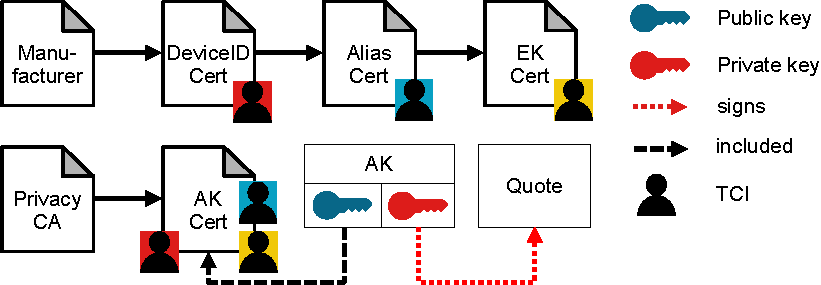
\includegraphics[width=1\linewidth]{figures/privacy-arch.pdf}
  \caption{The adapted architecture integrating privacy.} \label{fig:privacy_arch}
\end{figure}


We also need to transfer the DICE information from the old certificate chain to the new private one.
After performing the formerly described actions, the privacy CA creates a certificate vouching for that the AK was generated by an authentic TPM, hiding which exact TPM, even the manufacturer.
The privacy CA also copies each TCI of the old certificate chain into the AK certificate, as depicted in \autoref{fig:privacy_arch}.
The yielding private certificate chain is returned to the prover, who can forward it to a verifier without revealing its identity.

Whether the verifier trusts the firmware TPM is conducted in the same way as described in \autoref{subsec:trust_prover_tpm}, with the only difference is that the TCIs are all embedded into a single certificate, i.e., the AK certificate.
The verifier must also be able to trust the prover's quote as explained in \autoref{subsec:trust_quote_from_prover}.
For that, the verifier must trust the issuer of the AK certificate to have verified that the \ac{AK} is stored on an authentic TPM\@.
However, the privacy CA does not need to check whether AK is restricted.
This can be carried out by the verifier itself, as it continues to receive the TCI of the fTPM\@.

Ultimately, this adapted privacy architecture changes the statement a verifier can make from ``I am communicating with this authentic TPM in control of this EK'', to ``I am communicating with some authentic TPM in control of this AK.''
In other words, the verifier does not know exactly which TPM they are communicating with.
The privacy of the prover is guaranteed by the fact that the prover does not transmit any data derived from its \ac{UDS} to the verifier.

Nevertheless, privacy is not fully ensured because of the TCI values revealed to the verifier.
The order and values of the TCIs of an AK certificate might be sufficient to identify that it communicated with this particular prover before.
This can only be prevented by transferring the evaluation of the TCIs from the verifier to another entity, e.g., the privacy CA\@.
One possible realization is for the privacy CA to add to its policy that it will only certify AKs if they originate from a prover it considers trustworthy based on the TCIs it provided.
However, this makes the verifier dependent on another entity that decides whether the TCIs provided are trustworthy or not, which we consider undesirable.

We also want to highlight that the AK does not need to be a child of the EK, it does not even have to be part of the endorsement hierarchy.
In fact, it should not be part of the endorsement or platform hierarchy, since the TPM behaves differently when signing a quote depending on the hierarchy of the signing key~\cite{tpm20}.
If the signing key is part of the endorsement or platform hierarchy, the TPM assumes that privacy is irrelevant and embeds the TPM's firmware version, reset count, and restart count in plaintext in its generated quote.
This tuple might identify the TPM\@.
If the key is part of another hierarchy, this data is obfuscated by adding random offsets to each value, which is desirable if privacy is a concern.

% TODO: Maybe put somewhere earlier
% In general, endorsement keys represent device identities and are therefore privacy-sensitive.
% Our EK takes on the role of an attestation key, which has the task of signing attestation evidences.
% Although our EK does not represent the device identity, it does represent the identity of the shorter lived fTPM.
% This makes our EK also privacy-sensitive, since its generated signatures can be cross-referenced and then traced back to the according EK.
% Our approach has the advantage that we do not need a trusted third party, but trust the manufacturer of our trust anchor directly (DICE).
% In \autoref{sec:privacy}, an extension of our system is presented with privacy in mind.

% !TeX root = ../main.tex
% Add the above to each chapter to make compiling the PDF easier in some editors.

\chapter{Implementation}\label{chapter:implementation}

As explained in \autoref{sec:terminology}, from now on the term \acf{FWID} will be used instead of the previously used term \acf{TCI}.
Also keep in mind that while \ac{TEE} and \ac{REE} are the technology independent terms, we mainly use \acf{SW} and \acf{NW} here because of our implementation with Arm's TrustZone.

\section{Overview}


We run our implementation on Arm's Fixed Virtual Platform~(FVP)\footnote{\url{https://developer.arm.com/Tools\%20and\%20Software/Fixed\%20Virtual\%20Platforms}} which is a complete simulation of the Armv8-A architecture including TrustZone.

To do this, we use the software infrastructure provided by OP-TEE for various platforms, including FVP\@.
OP-TEE uses the TrustedFirmware-A~(TF-A)\footnote{\url{https://www.trustedfirmware.org/projects/tf-a/}} package from Arm as firmware boot components.
However, we mock their attestation, i.e., their Alias certificates are statically compiled into the binaries instead of being dynamically generated, as TF-A and FVP do not implement DICE\@.
The development efforts to implement that exceeds the benefits, as the concept can also be demonstrated with mocked certificates.
For that, only the certificates up to the OP-TEE~OS are mocked, including OP-TEE~OS's private key to sign the subsequent alias certificate, which is our EKcert.

Our implementation with compilation and running instructions can be found on GitHub.\footnote{\url{https://github.com/akorb/master-thesis-meta}}

\section{Boot chain}

The boot process is depicted in \autoref{fig:boot_chain}.
DICE is the root of trust, because incorrect behavior remains undetected and would jeopardize the security of our attestation process.

\begin{figure}[htpb]
  \centering
  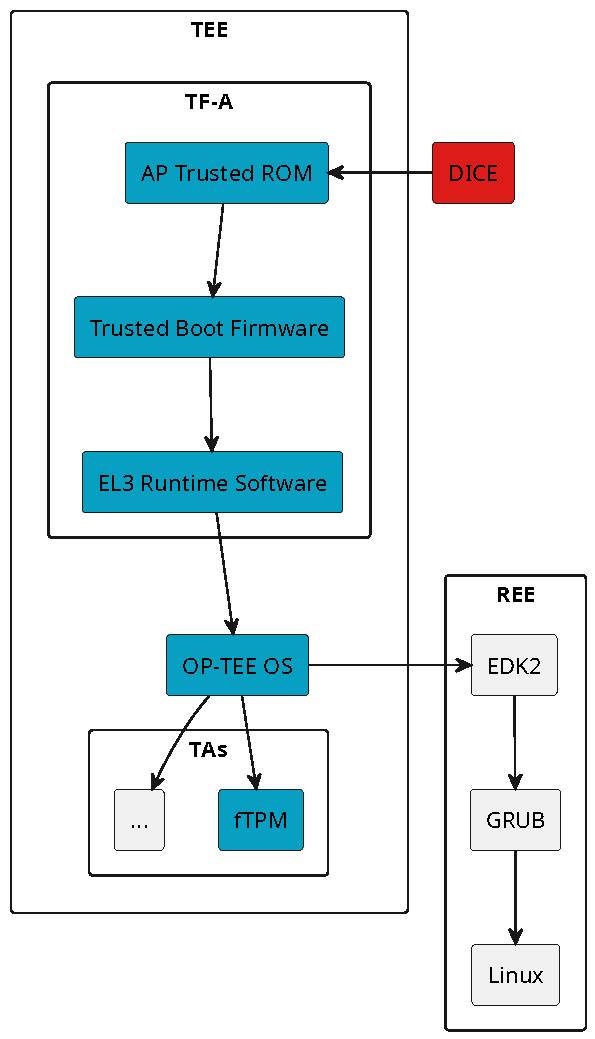
\includegraphics[width=0.8\linewidth]{figures/boot-chain.pdf}
  \caption{The boot chain of our system running in Arm's FVP\@. Blue: Represented by our yielding certificate chain. Red: Root of trust for verifier, and assumed to be present.}\label{fig:boot_chain}
\end{figure}



\paragraph{DICE}
Theoretically, the boot chain begins with the DICE hardware, but this is not included in FVP\@.
Therefore, we simply assume its presence by mocking the first few certificates of the yielding certificate chain.
Furthermore, it is independent hardware, and therefore, neither part of the TEE nor the REE\@.

\paragraph{TF-A}
After reset, the CPU executes within the \ac{SW}.
That is also the reason why boot software that is unaware of the separation between \ac{SW} and \ac{NW} are running in the \ac{SW}, as they never modify the execution environment of the processor.
This ensures that such systems have all expected privileges, which would be restricted in the \ac{NW}.
The Application Processor~(AP) Trusted ROM sets up the platform-specific exception vectors.
The Trusted Boot Firmware enables the MMU, performs the platform security setup, and other tasks.
The final component of TF-A---the EL3 Runtime Software---replaces the simple and rudimentary initialization performed by the AP Trusted ROM with more complete configurations by detecting the system topology, and enabling \ac{NW} software to function correctly.
It also provides the monitor which conducts the context switches between the \ac{SW} and the \ac{NW}.
More complete and detailed information can be found in the TF-A documentation.\footnote{\url{https://trustedfirmware-a.readthedocs.io/en/latest/design/firmware-design.html}}

\paragraph{OP-TEE~OS}
Just like an ordinary OS, OP-TEE~OS\footnote{\url{https://github.com/OP-TEE/optee_os}} initializes its functions offered to the user space of the \ac{SW}, i.e., the \acp{TA}.

\paragraph{Trusted Applications}

Our TA in focus is the firmware TPM\@.
We use the reference code\footnote{\url{https://github.com/microsoft/ms-tpm-20-ref/}} by Microsoft which implements a TPM, and the stub code, which provides and implements the interfaces required to be a TA of OP-TEE~OS\@.
The combination of the TPM code with the OP-TEE interfaces results in a \ac{fTPM}\@.
This fTPM only allows a single connection at any time, i.e., it prohibits concurrent access as this could lead to inconsistent states.
This also mirrors hardware TPMs, which are usually attached via serial buses like SPI to the processor.
Typically, the only entity that communicates with the fTPM is a Linux kernel module\footnote{\url{https://docs.kernel.org/security/tpm/tpm_ftpm_tee.html}}, so it is transparent to the user applications whether the TPM is implemented in firmware or hardware.
Note that TAs are not started automatically.
In fact, we are not aware of any function provided by OP-TEE~OS to register a TA to be started during the boot process. 
Instead, TAs are initialized the first time someone wants to interact with them.

\paragraph{EDK II}
TianoCore EDK II\footnote{\url{https://github.com/tianocore/edk2}} is the first component launched in the \ac{NW}.
It is a reference implementation of UEFI~\cite{UEFI} by Intel.

\paragraph{GRUB}
The GNU GRand Unified Bootloader\footnote{\url{https://www.gnu.org/software/grub/}} is a bootloader which is responsible for loading and transferring control to OS kernel software.

\paragraph{Linux}
The final component to boot is the Linux\footnote{\url{https://www.kernel.org/}} operating system.

\section{Firmware TPM initialization}

Initialization begins with the derivation of all secrets from the CDI\@.
Note that we mocked the CDI that would be passed from OP-TEE OS to the fTPM in practice.
However, OP-TEE OS does not implement DICE\@.

We use the Mbed TLS library\footnote{\url{https://mbed-tls.readthedocs.io/en/latest/}} providing cryptographic primitives for the derivation of the secrets, and also to build X.509 certificates.
Mbed TLS is already part of OP-TEE, and its functionality is modular and allows certain functionality to be activated or deactivated at a fine granular level.
Since the target machines are embedded devices with limited resources, the user should only activate the functions that he really needs.
We therefore had to activate some functions.

The formulas which derive secrets directly from the CDI (\autoref{eq:storage_key_formula}, \autoref{eq:eps_formula}) use a keyed-hash message authentication code~(HMAC) function.
This is inspired by the CDI derivation proposed in the DICE hardware requirements specification~\cite{dice-hardware-reqs}.
Actually, it proposes two functions to combine information to a new secret---a simple hash function, and a HMAC function.
It also recommends the HMAC function which calculation takes a little more time, but protects the CDI with twice the level than the simple hash function.
% https://nvlpubs.nist.gov/nistpubs/SpecialPublications/NIST.SP.800-57pt1r5.pdf (Table 3) shows that the HMAC version has roughly double security strength
This is backed by Jäger et al.~\cite{Jaeger2017}, and NIST SP 800--57~\cite{Barker2020}.
We declare the inner hash function used by the HMAC according to the required data size of the secret.
For example, for storage encryption, we use AES-128, and therefore, use the MD5 function to retrieve a key with a sufficient size.
Note that while MD5 is considered broken, HMAC in conjunction with MD5 is not~\cite{Bellare2006}.
The HMAC functions are seeded with a fixed character string that describes the purpose of the output secret.
% Formula from (2) in https://trustedcomputinggroup.org/wp-content/uploads/Hardware-Requirements-for-Device-Identifier-Composition-Engine-r78_For-Publication.pdf
\begin{align}
  \label{eq:storage_key_formula}
  K_{storage} &= HMAC_{MD5}(CDI,\ `DATA\ STORAGE\ KEY\text{'})\\
  \label{eq:eps_formula}
  EPS &= HMAC_{SHA512}(CDI,\ `ENDORSEMENT\ PRIMARY\ SEED\text{'})\\
  \label{eq:ek_formula}
  EK  &= KDF(EPS,\ EK_{template})
\end{align}

\begin{figure}[htb]
  \centering
  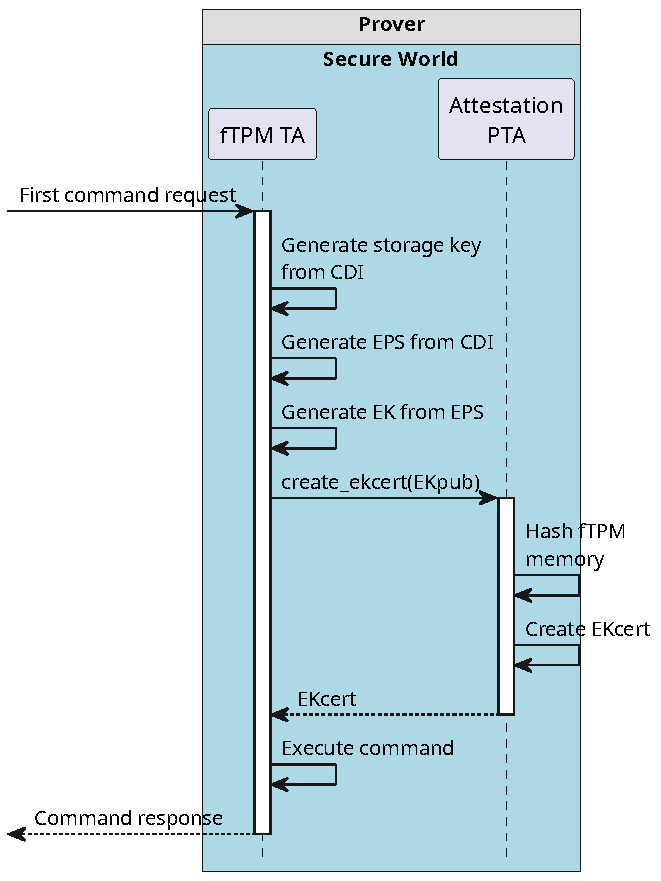
\includegraphics[width=0.62\linewidth]{figures/tpm-initialization.pdf}
  \caption{A UML sequence diagram describing the initialization of our firmware TPM\@.}\label{fig:ftpm_initialization}
\end{figure}


We must ensure we retrieve exactly the same EK as the TPM would generate by a \texttt{TPM2\_CreatePrimary} request with our EK template.
Therefore, we use the TPM internal functions to generate the EK\@.
The EK consists of a private and a public portion.
The private part never leaves the TPM, and the public portion is forwarded to OP-TEE's attestation PTA to be used as the subject key for EKcert, as shown by \autoref{fig:ftpm_initialization}.
A pseudo \ac{TA}~(PTA) provides the same interfaces as an ordinary TA, but runs in kernel mode within OP-TEE~OS instead of in user mode.
Therefore, it has more privileges than an ordinary TA\@.
The attestation PTA requires these privileges in order to read the memory of the calling TA, i.e., the fTPM TA, which is processed into the FWID that is finally embedded in the EKcert.
The attestation PTA hashes the memory pages of the calling TA that are constant, i.e., executable or read-only data.
Also, Microsoft's fTPM reference implementation does not contain separate configuration files, which simplifies the TCI generation of our fTPM by limiting it to the measurement of the fTPM itself.
The attestation PTA signs EKcert with OP-TEE's private alias key.
This key is mocked in our implementation.
Note that the fTPM has never access to the private alias key of OP-TEE OS, so it cannot fake its alias certificate/EKcert.

Another approach to measure the fTPM is to simply extract the hash embedded in its TA binary header.
A TA is an ELF binary wrapped in an OP-TEE specific format, which header contains a signature over all metadata and the payload, i.e., the ELF executable.
While it is simpler and faster, it does not attest a TA's dynamically linked libraries.
Although the reference firmware TPM does not link dynamically to any library, we use the attestation of the memory data to be more future-proof.

To embed the FWID into the EKcert, we use an X.509 extension defined by the DICE Attestation Architecture~\cite{TCGAttestation2021}---the TCB Info Evidence Extension.
It is defined formally in the ASN.1 description language.
Consequently, we use ASN1c\footnote{\url{https://github.com/vlm/asn1c}} to translate this formal definition to C~code.
In particular, we use a self-compiled version of ASN1c, since its last official release dates back to 2017, whereby its generated C~code throws various warnings with a modern C~compiler.
While it allows multiple FWIDs to be embedded into an X.509 certificate, our implementation only stores one into each alias certificate.
However, the privacy focused architecture explained in \autoref{sec:privacy} could leverage the possibility to store multiple FWIDs in the extension.
Each FWID consists of an identifier of the hash algorithm used, and the according digest.
We use SHA-256.

The resulting certificate generated by the attestation PTA is returned to the firmware TPM, which also has access to all preceding certificates.
In our implementation, these preceding certificates are simply mocked.

\section{Firmware TPM attestation}\label{sec:impl_ftpm_attestation}

\begin{figure}[htb]
  \centering
  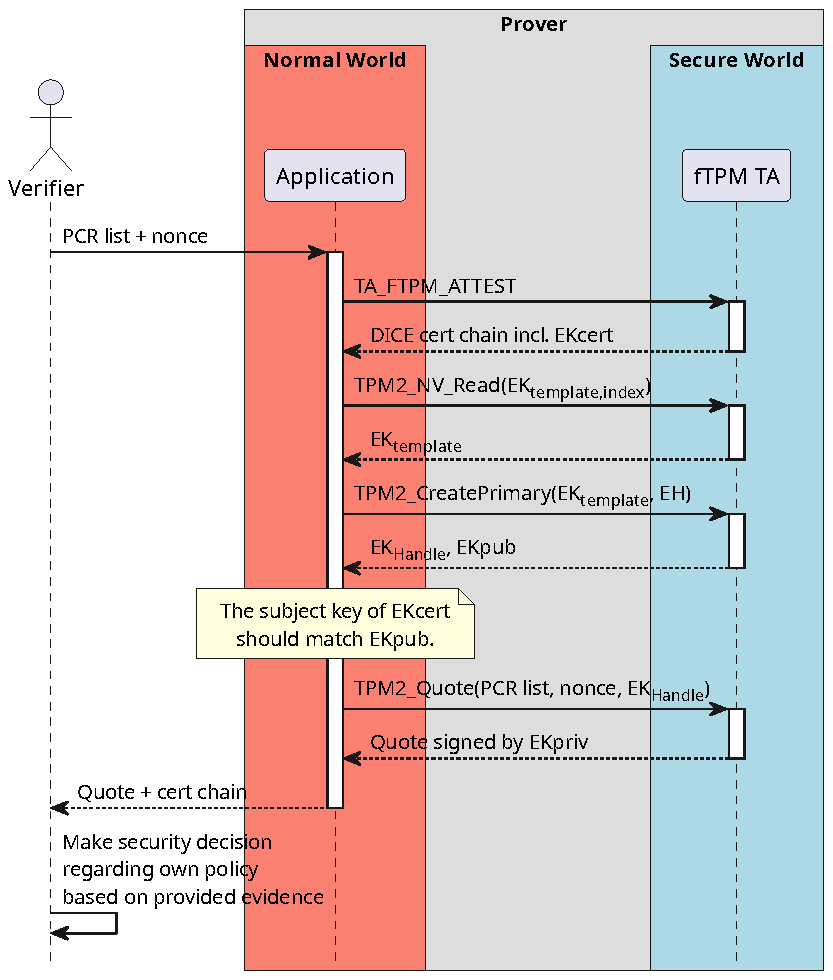
\includegraphics[width=0.74\linewidth]{figures/tpm-attestation.pdf}
  \caption{A UML sequence diagram describing the attestation of our firmware TPM\@.}\label{fig:ftpm_attestation}
\end{figure}


We added a new TA command called \texttt{TA\_FTPM\_ATTEST} to the \ac{fTPM} to obtain the entire certificate chain from any application.
Normally, this command is issued by the application that performs the prover part of the remote attestation.
We would like to emphasize that we do not refer to a new TPM command that would imply an extension of the TPM specification, but a new TA command that is intercepted by the OP-TEE stub code of the \ac{fTPM} and processed without the involvement of the TPM-specific core code.

Recall that we earlier described that the \ac{fTPM} TA only ever allows a single connection to it, which is usually a Linux module that provides the \texttt{/dev/tpm0} and \texttt{/dev/tpmrm0} nodes to communicate with the \ac{fTPM}\@.
We have therefore implemented the prover's side of the remote attestation with the ability to unload this Linux module before issuing \texttt{TA\_FTPM\_ATTEST}, and then load the Linux module again.

The prover's user space application starts with issuing the \texttt{TA\_FTPM\_ATTEST} command to the firmware TPM, as shown by \autoref{fig:ftpm_attestation}.
Consequently, it receives the certificate chain created by DICE with the EKcert as leaf certificate.

Afterwards, the prover wants the \ac{fTPM} to create the EK including its private portion.
To do this, it first reads the EK template from the non-volatile~(NV) storage of the fTPM, which was used earlier to create the EK part of the EKcert during the initialization process of the \ac{fTPM}.

Consequently, it then sends the template that has just been retrieved back to the TPM as part of the command \texttt{TPM2\_CreatePrimary}.
Since this command creates a primary key, no parent has be specified as the primary seed and the specified hierarchy is used instead.
So, we specify the endorsement hierarchy~(EH), which makes the TPM use the \ac{EPS} derived from the \ac{CDI} to generate the \ac{EK}\@.
The TPM returns a handle to the \ac{EK} just created, which is an integer, as well as the public part of the \ac{EK}\@.
The private part of the \ac{EK} is not returned, as this never leaves the TPM in plaintext.

Eventually, the prover wants to create a quote to establish trust to the prover's system state in the \ac{NW}, and to prove that it is in control of the EKpriv.
So, it issues the command \texttt{tpm2\_quote} to the TPM, specifying the PCR registers requested by the verifier, the verifier supplied nonce, and the handle to the EK just generated.

The prover's application handling the remote attestation is now in possession of the certificate chain, and a quote.
It transmits both to the verifier.
The verifier extracts the EKpub which is the subject key of the EKcert.
With that, it can verify the digital signature of the quote.
The ability of creating a quote with a fresh nonce proves the control of EKpriv by the fTPM\@.
Therefore, the verifier can trust that the certificate chain does not have been replayed, and it represents the device it communicates with.

In our implementation of the prover we do not send the TPM commands to the TPM ourselves, but use \texttt{tpm2\_createek~-t} and \texttt{tpm2\_quote} from the tpm2-tools.\footnote{\url{https://github.com/tpm2-software/tpm2-tools}}
Nevertheless, it executes these commands behind the scenes.
We also use \texttt{tpm2\_checkquote} in the verifier's implementation to check the signature of the quote, and to ensure that the nonce in the quote matches the nonce that the verifier has previously generated.

Note that the implementation just described assumes that the quote returned by \texttt{TPM2\_Quote} contains the values of the PCR registers.
While this was the case with TPM~1.2, this changed with version~2.0.
Instead, the resulting quote only contains a hash of the values of the requested PCR registers.
The corresponding plaintext PCR values are transmitted unprotected to the verifier.
After validating the quote, the verifier can check whether the hash of the plaintext PCR values computed by itself matches the PCR hash from the quote.
If this is the case, it can trust them.
This is also done by the tool \texttt{tpm2\_checkquote}.
We have omitted it from the previous explanation and \autoref{fig:ftpm_attestation} in order to focus on the important aspects.
For the sake of completeness and correctness, we mention it here anyway.

As a small note, we made sure that the property \texttt{tpmGeneratedEPS} of our fTPM is set to 1 as it indicates that the EPS was generated by the TPM~\cite{tpm}, which is the case in our implementation as it is derived from the CDI within the TPM\@.


\section{Creating and storing our EK template and certificate}
% \section{Adaption of the Endorsement Key}

The EK is a primary key, so it is derived from the EPS, and also a key template.
The template must be provided as part of the command \texttt{TPM2\_CreatePrimary} to the TPM\@.
The TPM can contain a template for an EK key, which shall be the template with which the EK part of the EKcert was created.
This is necessary to be able to reproduce the EK contained in the EK certificate so that the TPM can prove that this EK certificate corresponds to it by being able to generate the corresponding private key.

A TPM can save an EK template, but is not obliged to do so.
Then, the default template defined by TCG~\cite{tcg-ek} is used, dictating the \ac{EK} to be a restricted encryption key, since it is privacy-sensitive, and that it must be an RSA~2048 key.
As this is fitting for most TPM's, the definition of the default template removes the burden of most TPM's to provide the template.
It is then the duty of the entity communicating with the TPM to provide the default EK template, since it is unknown to the TPM itself.
Though, we extended our firmware TPM to be able to generate the default and our custom EK template within code, such that it can create the EK which it forwards to the OP-TEE~OS to create the EK certificate.

% The default template is not stored on the TPM, but it is part of the command triggering the key generation (\texttt{TPM2\_CreatePrimary}).
% Therefore, the TPM itself does not need to know what the default template is, since it is always provided by TPM-capable software.

We want to use the EK as a signing key to sign attestation data, i.e., a quote.
Hence, we need to deviate from the default EK template, and also provide our template within the NV of our fTPM\@.
We start with the default EK template and only modify the fields when necessary.
In total, we needed to change three aspects.
We declare the EK as a (i)~restricted signing key.
This also requires to specify a (ii)~signature scheme where we selected RSASSA-PKCS1-v1\_5~\cite{Jonsson2003} with SHA-256, and (iii)~no inner symmetric key as required by the TPM specification~\cite{tpm} for signing keys since they are not allowed to have any children keys, as a signing key cannot encrypt its children for storage outside the TPM\@.

% We create this EK template within the firmware TPM in code on its first launch after any reset.
This template will be generated within the TPM after each manufacturer reset, so it will be preserved even after an identity change and a subsequent reset of the \ac{fTPM}\@.
Thus, it is always present and stored in the NV index \texttt{0x01c00004} as defined by the TPM EK specification~\cite{tcg-ek} for RSA 2048 EK templates.
We set the attributes for this NV index as defined by the TPM PC Client specification~\cite{tcgPcClient}. % 4.5.2.1
Thereby, the EK template in the NV can only be written or deleted if a specific policy is fulfilled.
However, the policy is empty, which can never be fulfilled.
This results in a non-deletable EK template.
We also store the EKcert in the NV index \texttt{0x01c00002} as defined by the TCG EK Credential Profile~\cite{tcg-ek} with the same attributes as the respective template, so that it also cannot be deleted.
The template and certificate do not contain any sensitive material and can hence be read by anyone using the command \texttt{TPM2\_NV\_Read}.

Nevertheless, our \ac{fTPM} does not retrieve the EK template from the NV index to create the EK to subsequently forward it to the OP-TEE~OS to generate the EK certificate.
This would entail an indirection via the NV storage, which is not attested.
Instead, we explicitly use the EK template generated by code, which is attested via the fTPM's TCI\@.
% Ensure that the template generated by code is also directly used, instead of indirectly via unmeasured storages.
The NV storage is not attested as it is working data and not configuration data.
Hence, the fTPM's TCI would not only represent the fTPM's behavior, but also its stored data.
Since a TPM can store arbitrary data, this would explode the amount of TCI values that the verifier needs to know in order to derive the trustworthiness.
% However, the component right before the fTPM knows the fTPM's CDI, could generate the according symmetric key to decrypt the NV storage, and integrate the required NV values in the FWID\@.
% By baking the EK template generation in code which is already attested (and the code exists anyways), we prevent this complexity.

% The working data is not attested, since this would restrict the functionality of the fTPM\@.
% So, the an NV index is with ordinary TPM commands, providing the required policy/authentication is fulfilled.
% We consider this configuration as out-of-scope for attestation, for the former mentioned reason.
% In other words, it could be that everyone can change the NV index, where the template is stored.
% And in the subsequent boot, we would create a EKcert for it, without anything.
% Therefore, during EKcert creation, generate the template in code (which is attested), and use this directly.


\section{Times in certificates and systems}

In \autoref{tab:cert_comparison} we presented the restrictions the alias and the EK certificate specifications conduct on the valid times of the certificates.
Thereby, the period of validity of our certificates must be from a known time in the recent past, e.g., the component's build time, without expiration date.

We initially aimed for using the build time for the start of the validity period.
However, this turned out to be infeasible, since the guest machine in the FVP does not have internet access out of the box, and FVP also does not provide an option to use the time of the host.
While the host generates the mocked certificates, the FVP must continue the certificate chain and also check whether the current time falls within the validity period of the resulting certificates.
Therefore, the time of the host and the FVP guest would need to be synchronized manually, requiring unnecessary engineering effort.
Instead, we fix the times of the guest machine and the certificate's validity periods to pre-determined values.
This ensures that the FVP does not have to be configured for internet access which keeps the effort to launch the demonstration low, and results in a higher stability of the demonstration system.

We use \texttt{2023--07--25 00:00:00} as the start period for the certificates.
This date has no further meaning and was chosen arbitrarily at some point during development.
As required in the specifications, we indicate that the certificates do not have a well-defined expiration date, which is indicated by \texttt{9999--12--31 23:59:59}~\cite{Boeyen2008}.

The time of the guest machine is automatically set to \texttt{2023--08--02 11:46} with the Linux tool \texttt{date} at startup.
As before, this date has no further meaning.
It is only important that this date is after the start period of the certificates.

\section{Implementing encrypted storage}

Overall, the reference TPM's memory size has a size of 16,896 bytes, separated in a NV storage of 16,384 bytes, and the admin space of 512 bytes.
The admin space is reserved to persist defined data like the TPM's attributes, e.g., \texttt{tpmGeneratedEPS}.
The NV storage can store arbitrary data, e.g., the EK template, certificate, or an encryption key.
For example, Microsoft's BitLocker stores the encryption key for hard disk encryption in the NV storage.

The OP-TEE~OS manages storage in blocks.
It is only possible to write entire blocks, not partial blocks.
Therefore, little changes can be expensive to persist if the according block is big.
Hence, the OP-TEE specific code of the reference fTPM splits the memory size of 16,896 bytes in 512 bytes blocks resulting in \( 16{,}896 \div 512 = 33 \) blocks.

We consult the recommendations of the BSI~\cite{bsi-key-recommendations} to determine the encryption method.
Therefore, we use AES-128 in GCM mode to protect the data's confidentiality and integrity with an initialization vector~(IV) and tags of length 96 bits.
These are the recommended minimum sizes that we have chosen in order to spare resources.
There is one IV and tag for each block, and a key of 128 bits which results in a storage overhead of 808 bytes as shown in \autoref{eq:memory_overhead}.
\begin{equation}
  \label{eq:memory_overhead}
  \frac{33 \times (96 + 96)\ \text{bits} + 128\ \text{bits}}{8} = 808\ \text{bytes}
\end{equation}

The IVs are randomized on every write event.
On any mismatch between the stored tag and the tag produced during decryption, the firmware TPM is reset. 

The data is loaded from the hard disk and then decrypted only at startup time.
And it is written only during shutdown of the TPM or if a command modifies the TPM's storage.
As data is mainly written to the TPM during the provisioning time and only read during daily use, we expect that the impact on performance will be small.

\section{Isolating storage of fTPM in OP-TEE}

The data of the individual \acp{TA} must be saved somewhere permanently.
The OP-TEE~OS stores them in the \ac{REE} file system.
Hence, this data must be protected.
OP-TEE encrypts the secure storage files before sending them to the \ac{REE} using a pseudo-randomly generated key---the File Encryption Key~(FEK).
It is stored in the metadata of the corresponding file, encrypted with a key unique to each \ac{TA}---the \ac{TA} Storage Key~(TSK). % (https://optee.readthedocs.io/en/latest/architecture/secure\_storage.html#trusted-application-storage-key-tsk).
It is derived from the Secure Storage Key~(SSK), which is unique to the device.
% \begin{itemize}
%   \item SSK:\ Unique per device
%   \item TSK:\ Unique per TA
%   \item FEK:\ Unique per file
% \end{itemize}
\begin{align}
  % \label{eq:ssk_formula}
  % SSK &= HMAC_{SHA256}(HUK,\ Chip\ ID\ \|\ `static\ string\text{'})\\
  \label{eq:tsk_formula}
  TSK &= HMAC_{SHA256}(SSK,\ TA_{UUID})\\
  \label{eq:fek_formula}
  FEK &= decrypt_{TSK}(file_{metadata})\\
  file_{plain} &= decrypt_{FEK}(file_{cipher})
\end{align}
% where HUK is a hardware unique key, and the chip ID a UUID unique to the hardware, possibly derived from the HUK\@.
% More details can be found in OP-TEE's documentation\footnote{\url{https://optee.readthedocs.io/en/latest/architecture/porting\_guidelines.html}}.

\autoref{eq:tsk_formula} shows that the TSK depends only on the SSK and the TA's UUID\@.
As said, the SSK is same for the whole device and hence for every TA, and the \( TA_{UUID} \) is public.
A close look reveals that other TA's on the same device could therefore use the publicly available UUID to generate the fTPM's TSK and consequently, decrypt the FEKs of the fTPM's files and access private data of the fTPM\@.
However, this is prevented by our integration of an additional storage key, which encrypts the data before it is sent to the OP-TEE~OS\@.

The TEE specification offers an ultimate solution for that on the conception level of the trusted OS without requiring a manual encryption step in the TA itself.
It is defined in the TEE Management Framework~\cite{GP_ManagementFramework}, which offers the possibility of grouping TAs into domains and subdomains, whereby only TAs in the same domain or subdomain can potentially decrypt each other's data.
However, as of time of writing, this is not implemented in OP-TEE~OS yet.

\section{Technical obstacles}

\subsection{tpm2-tools}

As mentioned earlier, we use the \texttt{tpm2\_checkquote} tool to verify the prover's quote on the verifier's side.
However, this tool fails to perform an important check to ensure that the quote was generated by the TPM and not externally.
This poses a major security risk.
We have reported this to the authors of the tpm2-tools via the recommended channel.\footnote{\url{https://github.com/tpm2-software/tpm2-tools/security/advisories/GHSA-5495-c38w-gr6f}}

% \paragraph{RSASSA-PSS vs. RSASSA-PKCS1-v1\_5}
We would have liked to use RSASSA-PSS which is formally proven to be secure over RSASSA-PKCS1-v1\_5.
RFC 8017 even requires RSASSA-PSS for new applications~\cite{Moriarty2016}.
However, it is not fully supported by the tpm2-tools, yet.\footnote{\url{https://github.com/tpm2-software/tpm2-tools/issues/3283}}

The tool \texttt{tpm2\_createek} did not adhere to the TPM specification when it created the EK with a template from the NV storage of the TPM\@.
A template always contains a nonce, but it can be overwritten by storing another nonce in a specifically defined NV index.
We did not want to deviate from the standard nonce, which is a buffer of 256~bytes all set to 0.
Therefore, we did not write a nonce to the NV index, and only the EK template, which conforms to the TPM specification~\cite{tcg-ek}.
However, \texttt{tpm2\_createek} expected a template \emph{and} a nonce to be present.
We ended up writing an empty nonce in the according NV index of the firmware TPM with the sole aim of circumventing this problem.
Later, the maintainers of the \texttt{tpm2-tools} fixed it.\footnote{\url{https://github.com/tpm2-software/tpm2-tools/issues/3278}}
Then, it turned out that this tool has another bug that caused the address of the nonce  to be used instead of the actual nonce.
We fixed this issue.\footnote{\url{https://github.com/tpm2-software/tpm2-tools/pull/3280}}


\subsection{OP-TEE}

% Build

Initially, it failed to follow the official documentation to create the complete software ecosystem with the reference firmware TPM enabled.
Eventually, we determined the problem and fixed it.\footnote{\url{https://github.com/OP-TEE/optee_os/issues/6111}}

% Persistence

It was important for us to also test whether our system behaves as expected if the CDI changes.
For that, we needed to persist the storage of the firmware TPM between launches of the FVP to modify the CDI during its downtime.
However, the FVP version required to accomplish this turned out to freeze when the necessary functionality was activated.
It took extensive debugging efforts to find a workaround.\footnote{\url{https://github.com/OP-TEE/optee_os/issues/6162}}

The OP-TEE~OS provides a libc library which implements only subset of the C standard library.
Its authors copy code of the newlib\footnote{\url{https://sourceware.org/newlib/}} to their libc on-demand when required.
Unfortunately, the code generated by the asn1c project expects functions not part of OP-TEE's libc.
Fortunately, these functions were not critical and could be removed manually in a reasonable amount of time.

\subsection{Firmware TPM TA}

We have enabled a compilation option offered by the fTPM TA which appears not to have been thoroughly tested.
When the option is enabled, the TPM uses code written specifically for the OP-TEE platform to generate the EPS\@.
This resulted in a crash of the fTPM during startup.
We fixed the bug and opened a pull request for the fix to be merged upstream.\footnote{\url{https://github.com/microsoft/ms-tpm-20-ref/pull/98}}

Eventually, we did not use this code.
Nevertheless, this bug was found in the context of this thesis, and hence, we want to mention it here.

% !TeX root = ../main.tex
% Add the above to each chapter to make compiling the PDF easier in some editors.

\chapter{Discussion}\label{chapter:discussion}

\section{Assessment of the fulfillment of requirements}

\subsection{Security requirements}

\subsection{Attestation process requirements}

% Definitions

\ac{TCG} defines as part of their Trusted Attestation Protocol \cite{tap} the requirements for an attestation process to provide assurance to a verifier that it is (i) accurate, (ii) interpretable, and (iii) attributable.

(i) Accurate attestation data represents the actual state of the device.
This includes freshness, i.e., the data is not replayed and does not represent an old, outdated state of the device.

(ii) Intuitively, the data must be interpretable by the verifier.
In other words, the verifier must be able to derive a decision about the trustworthiness of the prover based on the attestation data.

(iii) It must be possible to assign the attestation data to a specific device, i.e., it must be verifiable that the attestation data originates from the prover.

% Why they are reached

\section{Higher level protocols' compatibility}

\section{Implications of missing privacy}

% An attacker could use the TCIs to find the exact version of the running software and match this to known vulnerabilities of this version.
% See: https://www.rfc-editor.org/rfc/rfc9334.html#section-11

\section{Hardware knowledge dependency}
% Or hardware-agnostic?

% Comparison to RATS architecture
% For RATS: Our system would be integrated by the verifier to establish trust into the fTPM, the relying party wouldn't need to know about it
% For us: verifier = relying party: full burden, needs to know everything
% but required for a (mostly) independent attestation.
% Otherwise trust relationship between verifier and relying party required
% See also Introduction of https://dl.acm.org/doi/10.1145/3600160.3600171

% See abstract of https://www.ietf.org/archive/id/draft-birkholz-rats-corim-01.html

\section{Hardware requirements DICE + fTPM vs TPM}

% Does it even make sense? (Price wise, maybe energy wise)

\section{Requires reproducible builds}

% The reference values have to come from somebody. Huge burden to the verifier, see paper of Simon for potential improvement

\section{Personal opinion about developed system}

% Maybe too complex?
% Bad feeling about this?
% Benefit bigger than effort?

% !TeX root = ../main.tex
% Add the above to each chapter to make compiling the PDF easier in some editors.

\chapter{Future Work and Conclusion}\label{chapter:future_work_and_conclusion}

\section{Future Work}

The logical consequence is the implementation of our solution on real hardware instead of in a simulation environment such as FVP\@.
This allows the interaction with the hardware to be verified, especially with an RPMB partition that requires hardware support.
In addition, the impact of our solution on the performance of the system can then be measured in practice.
This is especially interesting since we integrate another storage encryption.

Although it makes sense to show our solution on Arm hardware first, we are, as mentioned, not limited to it.
Therefore, a future work is to concretize the description of our implementation for TEE technologies other than Arm, e.g. Intel~SGX\@.

The system we propose can also be transferred from the DICE architecture to other technologies that also perform firmware measurements.
A new technological framework that generalizes DICE is Caliptra~\cite{caliptra}.
It is based on the concept of DICE, but is not limited to it.

As mentioned in \autoref{sec:arch_overview}, RPMB's rollback protection only protects against attacks from outside the TEE\@.
We would like to establish a design that tightens the rollback protection from the trust of the entire TEE to the identity of the fTPM\@.
This can probably be achieved by encrypting the metadata stored on the RPMB with the storage key derived from the identity of the fTPM, i.e., its CDI, before sending it to the RPMB\@.
This must be implemented in the trusted operating system and not in the fTPM TA, as the trusted operating system normally manages the metadata.

Furthermore, our solution does not protect against runtime attacks on the fTPM\@.
In general, trusted applications in a TEE are not resistant to security problems caused by programming errors, e.g., buffer overflow attacks.
Therefore, remote attestation of the control flow integrity of the fTPM may be a desired function.
Displaying the current state of the fTPM instead of its identity at boot time would be a useful extension to our solution.

\section{Conclusion}

In this work, we have proposed a novel remote attestation scheme to establish trust in a firmware TPM\@.
fTPMs cannot be trusted based on their isolated identity alone, as their underlying software components are also security relevant, unlike dedicated TPMs which are a separate chip.
We therefore use the DICE as a hardware root of trust and measure each component during the boot process up to the fTPM\@.
The verifier can thus learn the measurements of the corresponding components and decide whether they are classified as trustworthy.
These measurements are transmitted from the prover to the verifier in the form of certificates.
Since it is in the nature of certificates that they are not considered secret and can therefore be easily replayed by malicious provers, the verifier must ensure that the certificates correspond to the device he is communicating with.
This is not directly ensured by our system, but should be part of the attestation protocol that runs atop of our system, e.g., the fTPM, which attests the state of the system with a quote.
To do this, the prover must prove that he has the private key that corresponds to the public key part of the certificate that describes the firmware TPM\@.
These keys are unique for the identity of the device (the \ac{UDS}) and the identities of the individual components (the TCIs) and therefore cannot be generated by other, potentially malicious, verifiers.
We concluded the presentation of our system with an explanation of a proof-of-concept implementation and a discussion of the feasibility, caveats and limitations of the system.

We believe that our system is an important step towards the independence of the manufacturer of the firmware TPM and its upstream software, whereas today provers trust a single manufacturer who is assumed to have provided all these components.
Our system also creates a hardware root of trust for the firmware TPM which, as the name suggests, cannot be provided by the fTPM as it is a software component.
In contrast, dedicated TPMs are capable of acting as a hardware root of trust.
Our system closes this gap.


\appendix{}

\microtypesetup{protrusion=false}

\addchap{Abbreviations}
\begin{acronym}
	\itemsep-.25\baselineskip
	% General
	\acro{TUM}[TUM]{Technical University of Munich}
	\acro{CA}[CA]{Certificate Authority}
	\acro{HSM}[HSM]{Hardware Security Module}
	\acro{RTM}[RTM]{Root of Trust for Measurements}
	\acro{SRTM}[S-RTM]{static \ac{RTM}}
	\acro{DRTM}[D-RTM]{dynamic \ac{RTM}}

	% TPM
	\acro{TPM}[TPM]{Trusted Platform Module}
	\acro{fTPM}[fTPM]{firmware TPM}
	\acro{dTPM}[dTPM]{discrete TPM}
	\acro{TCG}[TCG]{Trusted Computing Group}
	\acro{PCR}[PCR]{Platform Configuration Register}
	\acro{EPS}[EPS]{Endorsement Primary Seed}
	\acro{EK}[EK]{Endorsement Key}
	\acro{AK}[AK]{Attestation Key}

	% DICE
	\acro{DICE}[DICE]{Device Identifier Composition Engine}
	\acro{TCB}[TCB]{Trusted Computing Base}
	\acro{TCI}[TCI]{TCB Component Identifier}
	\acro{FWID}[FWID]{Firmware identifier}
	\acro{UDS}[UDS]{Unique Device Secret}
	\acro{CDI}[CDI]{Compound Device Identifier}

	% TEE
	\acro{TEE}[TEE]{Trusted Execution Environment}
	\acro{REE}[REE]{Rich Execution Environment}
	\acro{NW}[NW]{Normal World}
	\acro{SW}[SW]{Secure World}
	\acro{TA}[TA]{Trusted Application}
\end{acronym}

\listoffigures{}
\listoftables{}
\microtypesetup{protrusion=true}
\printbibliography{}

\end{document}
